\chapter{Benchmarking}
\label{sec:benchmarking}

\section{Goal}
\section{Experimental Setup}

\begin{landscape}
\begin{table}[p!]
\begin{adjustbox}{width=19cm}
\rowcolors{2}{gray!13}{white}
\begin{tabular}{l|ll|p{46mm}p{67mm}}
\rowcolor{gray!26}
Name & Connector & Data Type & Goal & Description \\

\hline
seq-fifo & fifo1 & Integer & Tease out Proto overhead & alternate between putting and getting on single thread. measure RTT. Repeat for different sizes of data. Compare overhead to std::spsc channel \\

SIMO clone & N-replicator & BigClonable & check if getters are effectively cloning in parallel & repeatedly clone from a single putter in parallel \\

SIMO copy & N-replicator & BigCopyable & check if copying saves a lot of time vs cloning & repeatedly copy from a single putter in parallel \\

MO clone & N-keeper & BigClonable & Check if waiting for putter adds significant time & repeatedly clone from a memcell \\

counting & binary counter & BigClonable & Check how effective the refcounting is & binary counter circuit, moving memory between cells a hell of a lot. not much firing \\

MO fine & N-keeper fine & BigClonable & Check if coordinator is the bottleneck & have one rule per getter. each readiness causing a firing. \\

bitsets & N-keeper fine & BigClonable & fire every time, but after N-1 false guard evals by bitsets & N-keeper where only the last port and rule are active. effectively have to traverse all these dead rules each time \\

hashsets & N-keeper fine & BigClonable & check if the bitsets themselves helped & repeat bitset experiments, but modify Reo-rs to use stdlib hashsets instead \\

transform & transformer & int, float & overhead of createfromcall & \\

filter & filter & int & & \\

router & router & int & & \\

parallel & parallel & BitCopyable & concoct a scenario where data is moving in parallel as much as possible. & 

\end{tabular}
\end{adjustbox}
\caption[TODO]{TODO}	
\end{table}
\end{landscape}

\section{Results}

\subsection{Port Operation Overhead}
Figure~\ref{fig:exper_rtt} shows RTT through a simple FIFO on a single thread. compared to spsc channel.
\begin{figure}
	\centering
	\makebox[\textwidth][c]{
		\begin{subfigure}[b]{0.63\textwidth}
			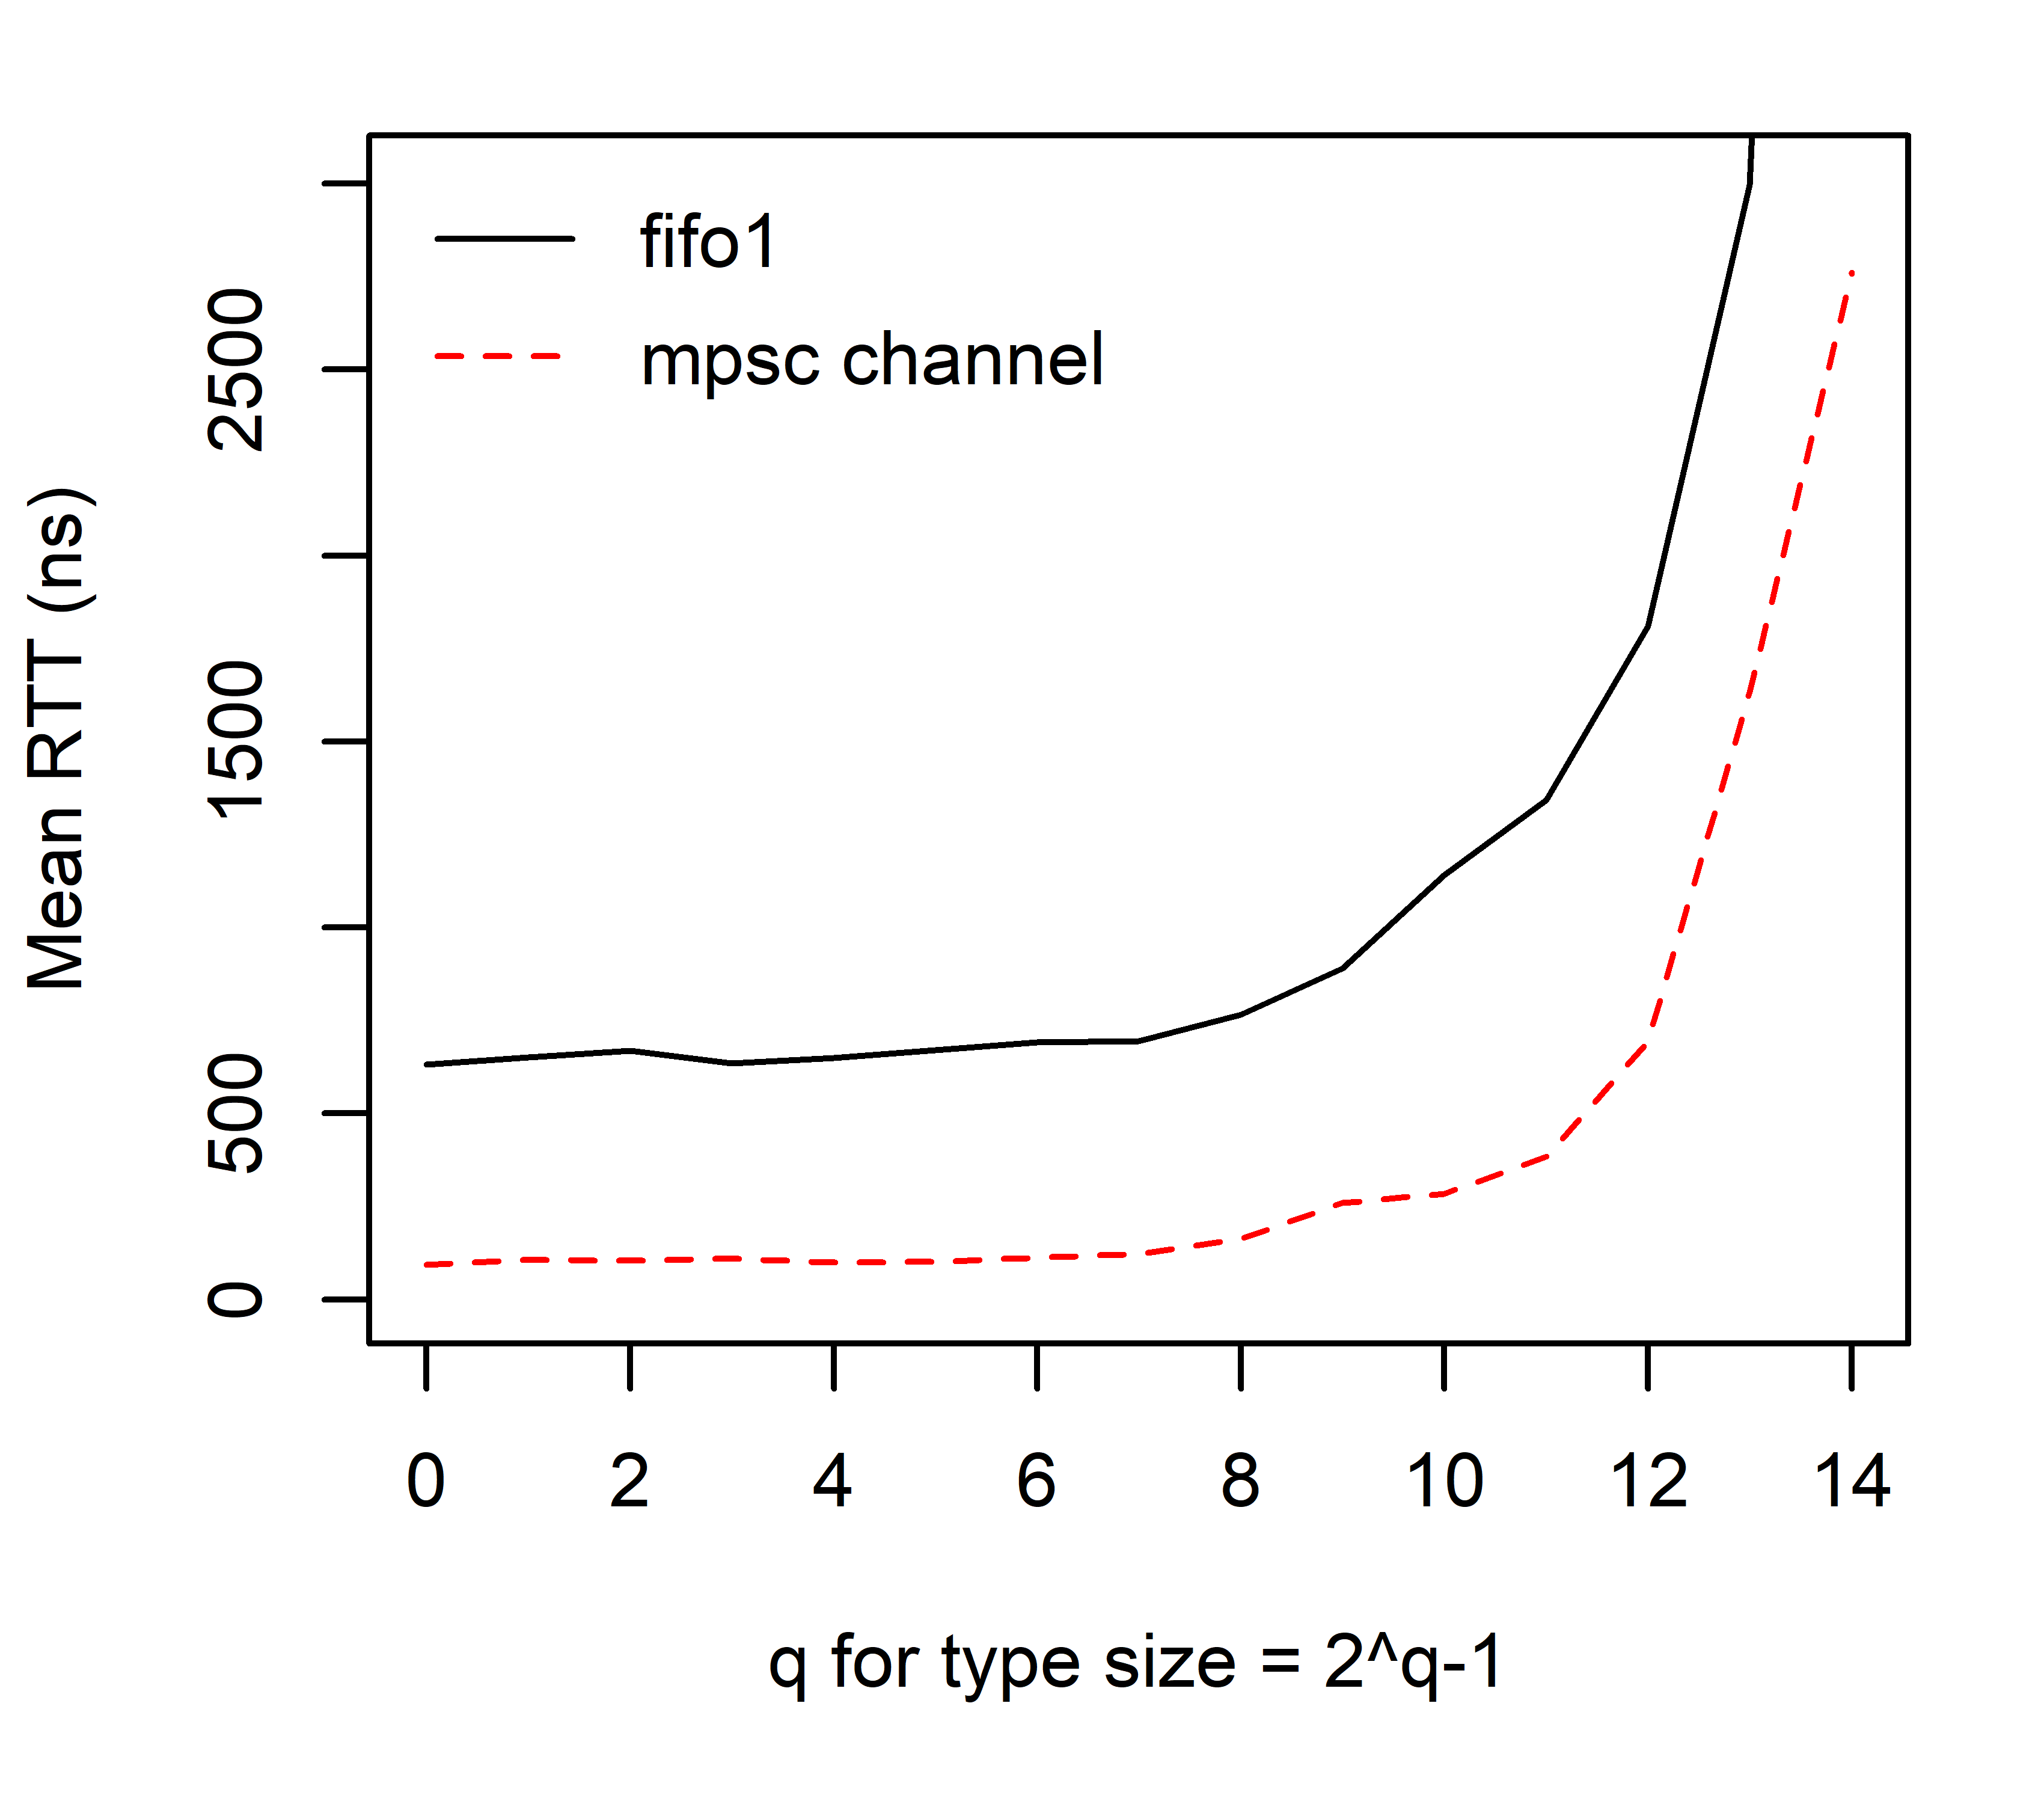
\includegraphics[width=\textwidth]{experiments/rtt_0.png}
			\caption{}
			\label{fig:exper_rtt_0}
		\end{subfigure}%
		\begin{subfigure}[b]{0.63\textwidth}
			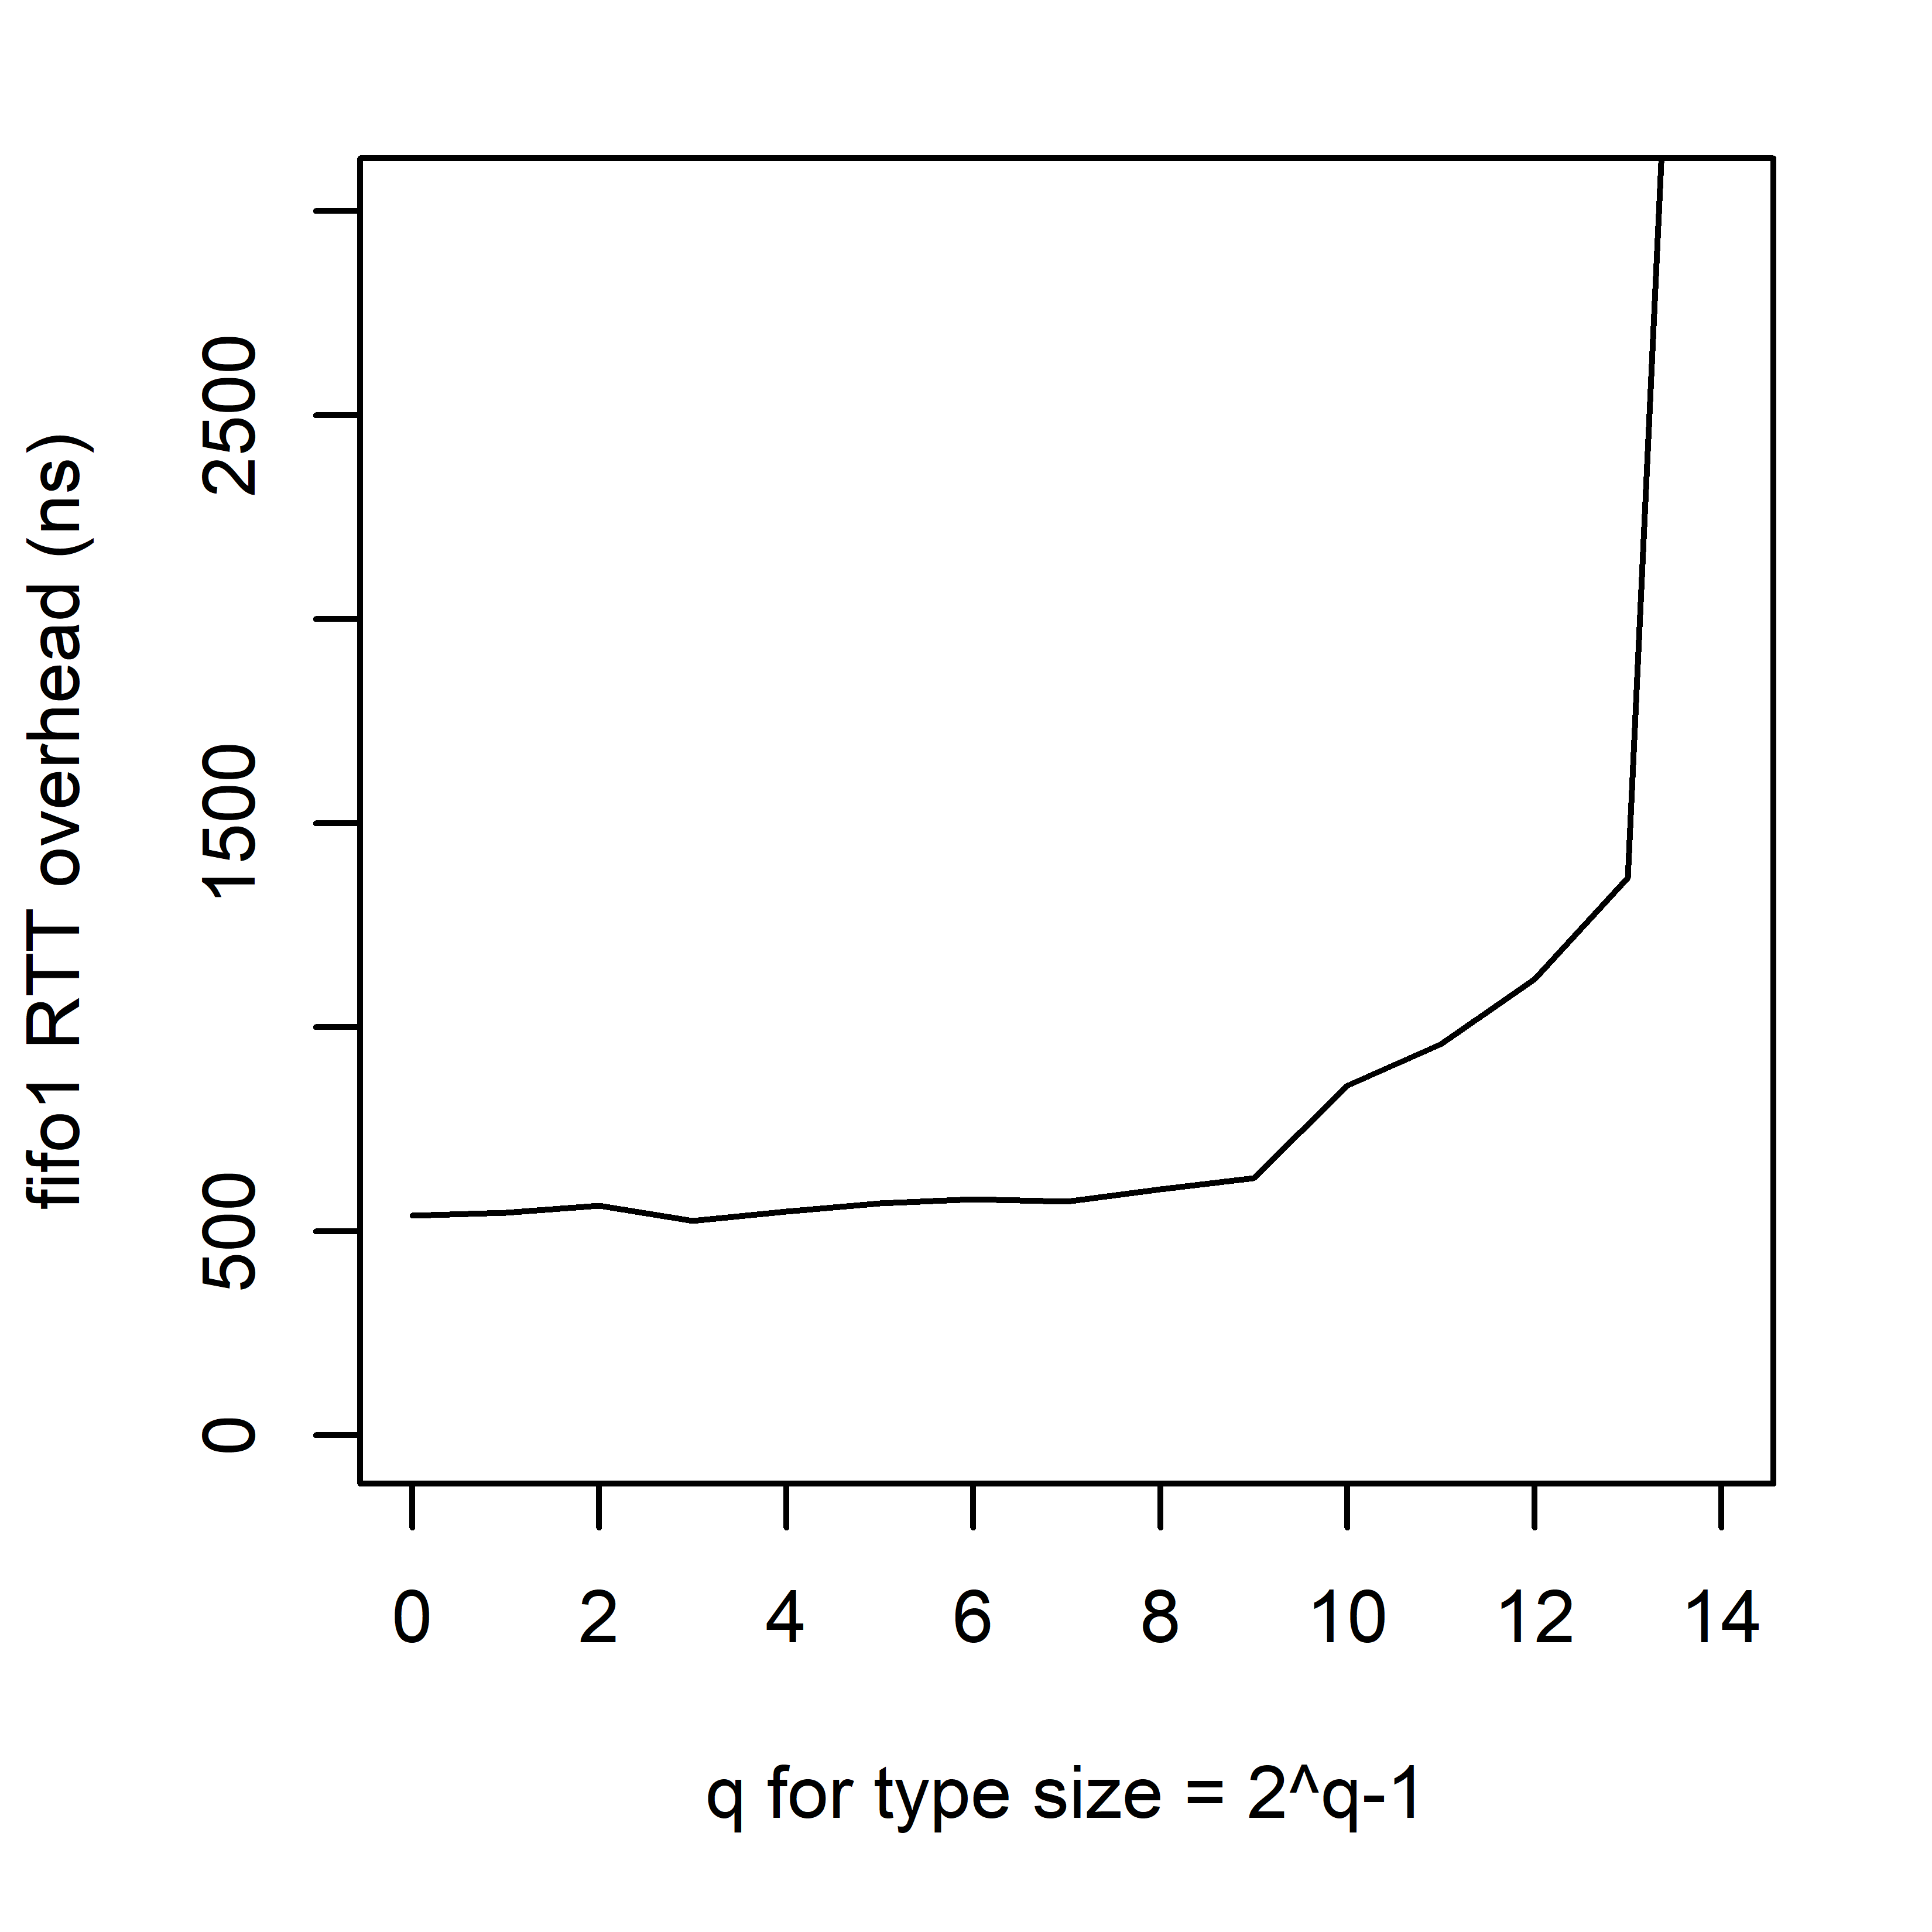
\includegraphics[width=\textwidth]{experiments/rtt_1.png}
			\caption{}
			\label{fig:exper_rtt_01}
		\end{subfigure}%
	}
	\caption[TODO]{TODO.}
	\label{fig:exper_rtt}
\end{figure}


Figure~\ref{fig:simo_copy} shows how it works with a multithreaded replicator connector. observe how the time taken increases with larger data as less fits in the cache. observe that the contention on the atomics (hardware locks) causes there to be superlinear overhead?? not sure what that's about. but observe that it does go down the larger the data becomes, showing that getters are able to get more effectively in parallel
\begin{figure}
	\centering
	\makebox[\textwidth][c]{
		\begin{subfigure}[b]{0.63\textwidth}
			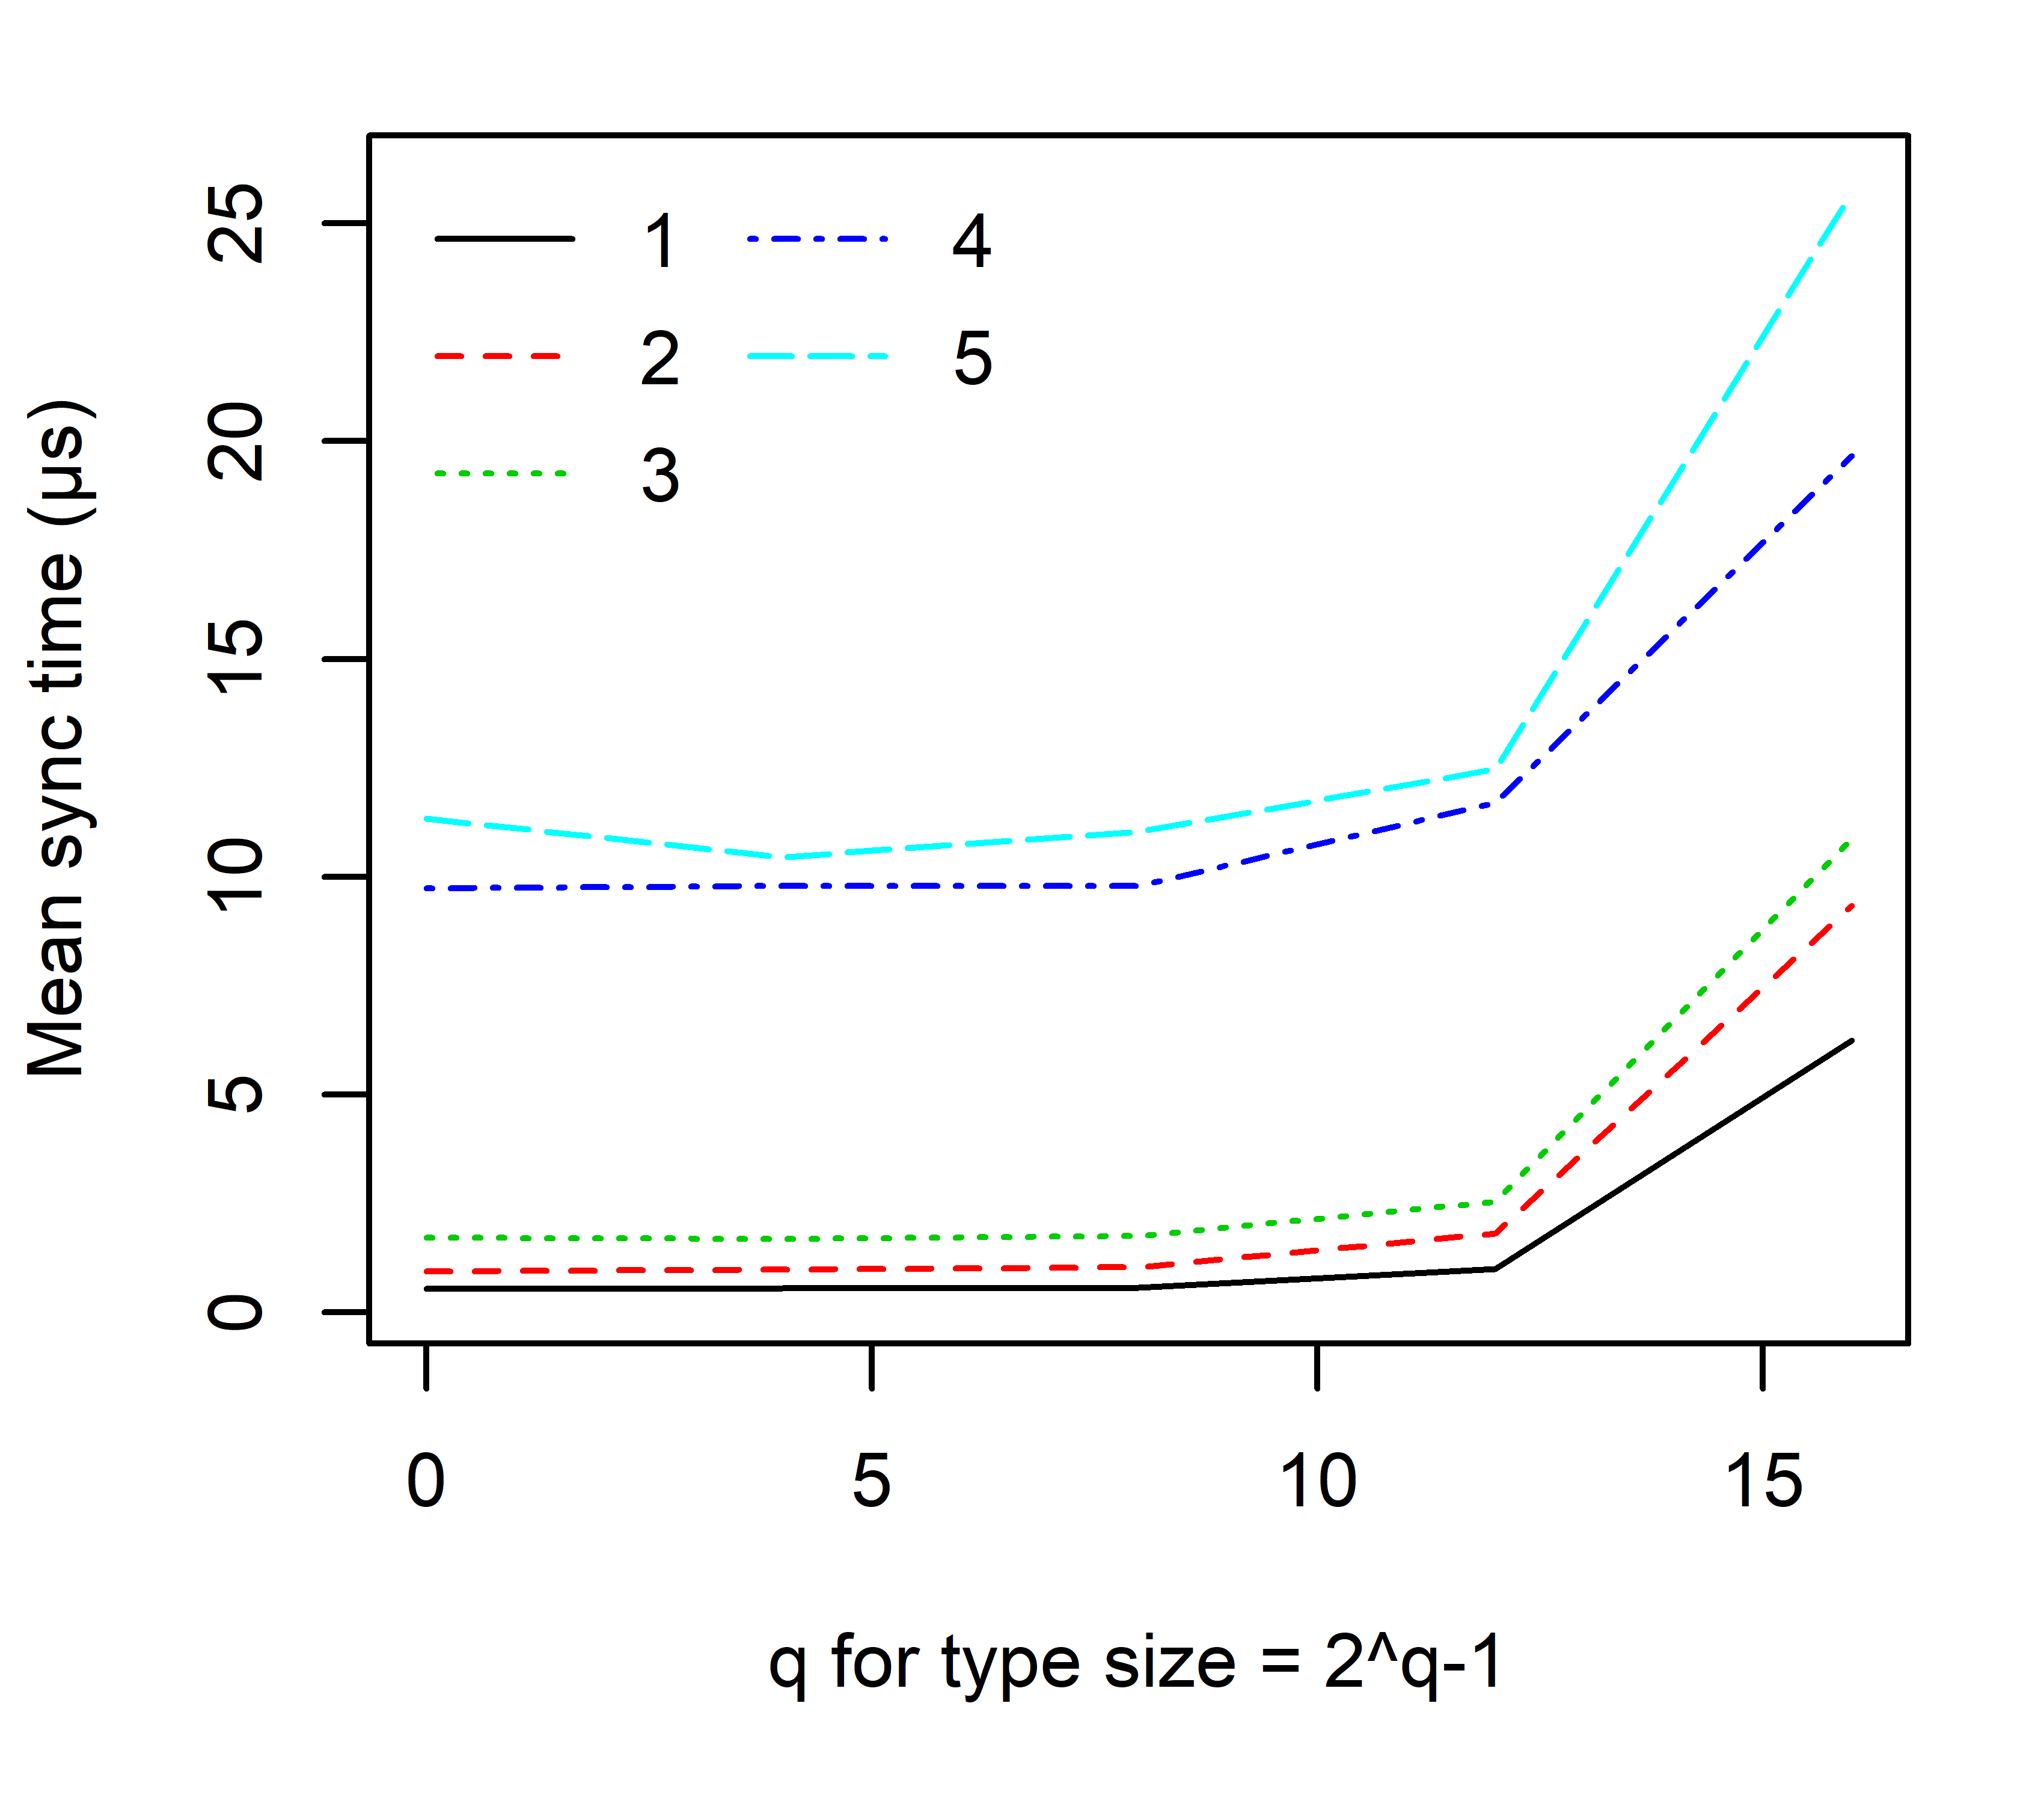
\includegraphics[width=\textwidth]{experiments/simo_copy_0.png}
			\caption{}
			\label{fig:simo_copy_0}
		\end{subfigure}%
		\begin{subfigure}[b]{0.63\textwidth}
			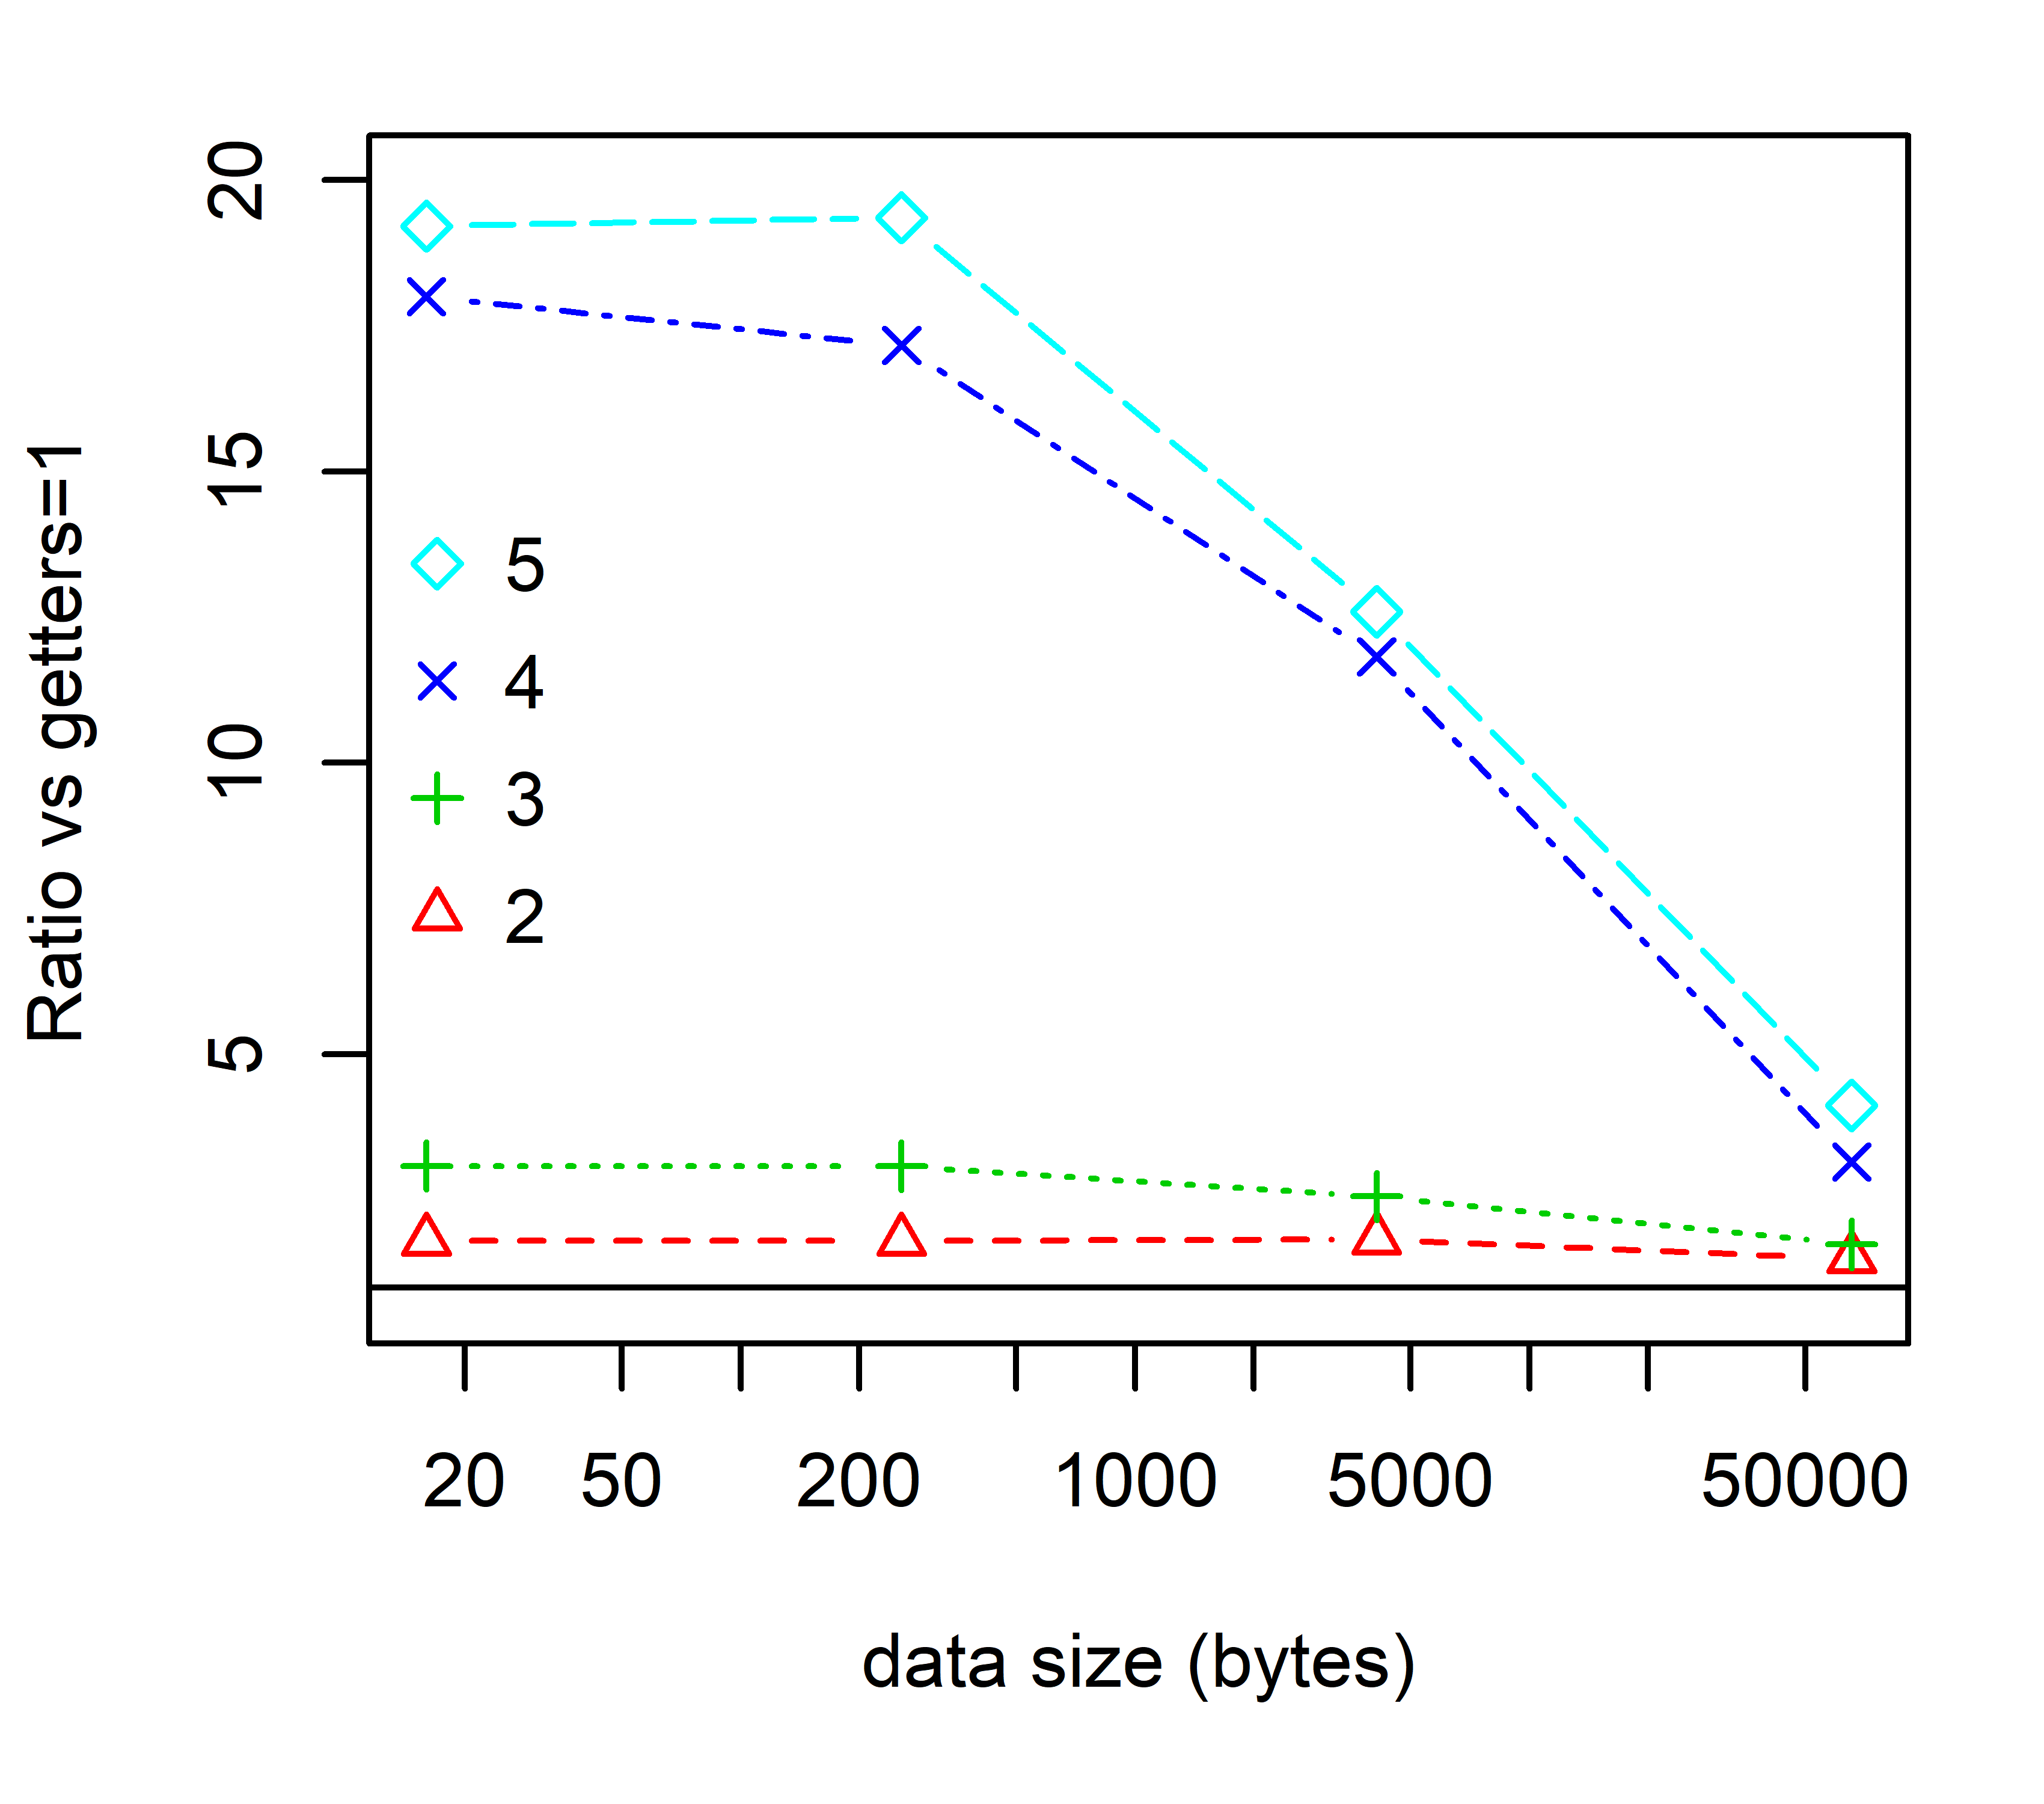
\includegraphics[width=\textwidth]{experiments/simo_copy_1.png}
			\caption{}
			\label{fig:simo_copy_1}
		\end{subfigure}%
	}
	\caption[TODO]{TODO.}
	\label{fig:simo_copy}
\end{figure}

Figure~\ref{fig:clone_compete} shows how long interactions take with N getters with a value that cannot be copied. observe the large jump from 1 to 2, as one is the mover. effectively when there is only one getter, no cloning is necessary. When the single-getter case is ignored, we see that larger numbers of getters converge on a ratio of time taken = 1 the larger the data, seen in Figure~\ref{clone_compete_3}.
\begin{figure}
\centering
\makebox[\textwidth][c]{
	\begin{subfigure}[b]{0.63\textwidth}
		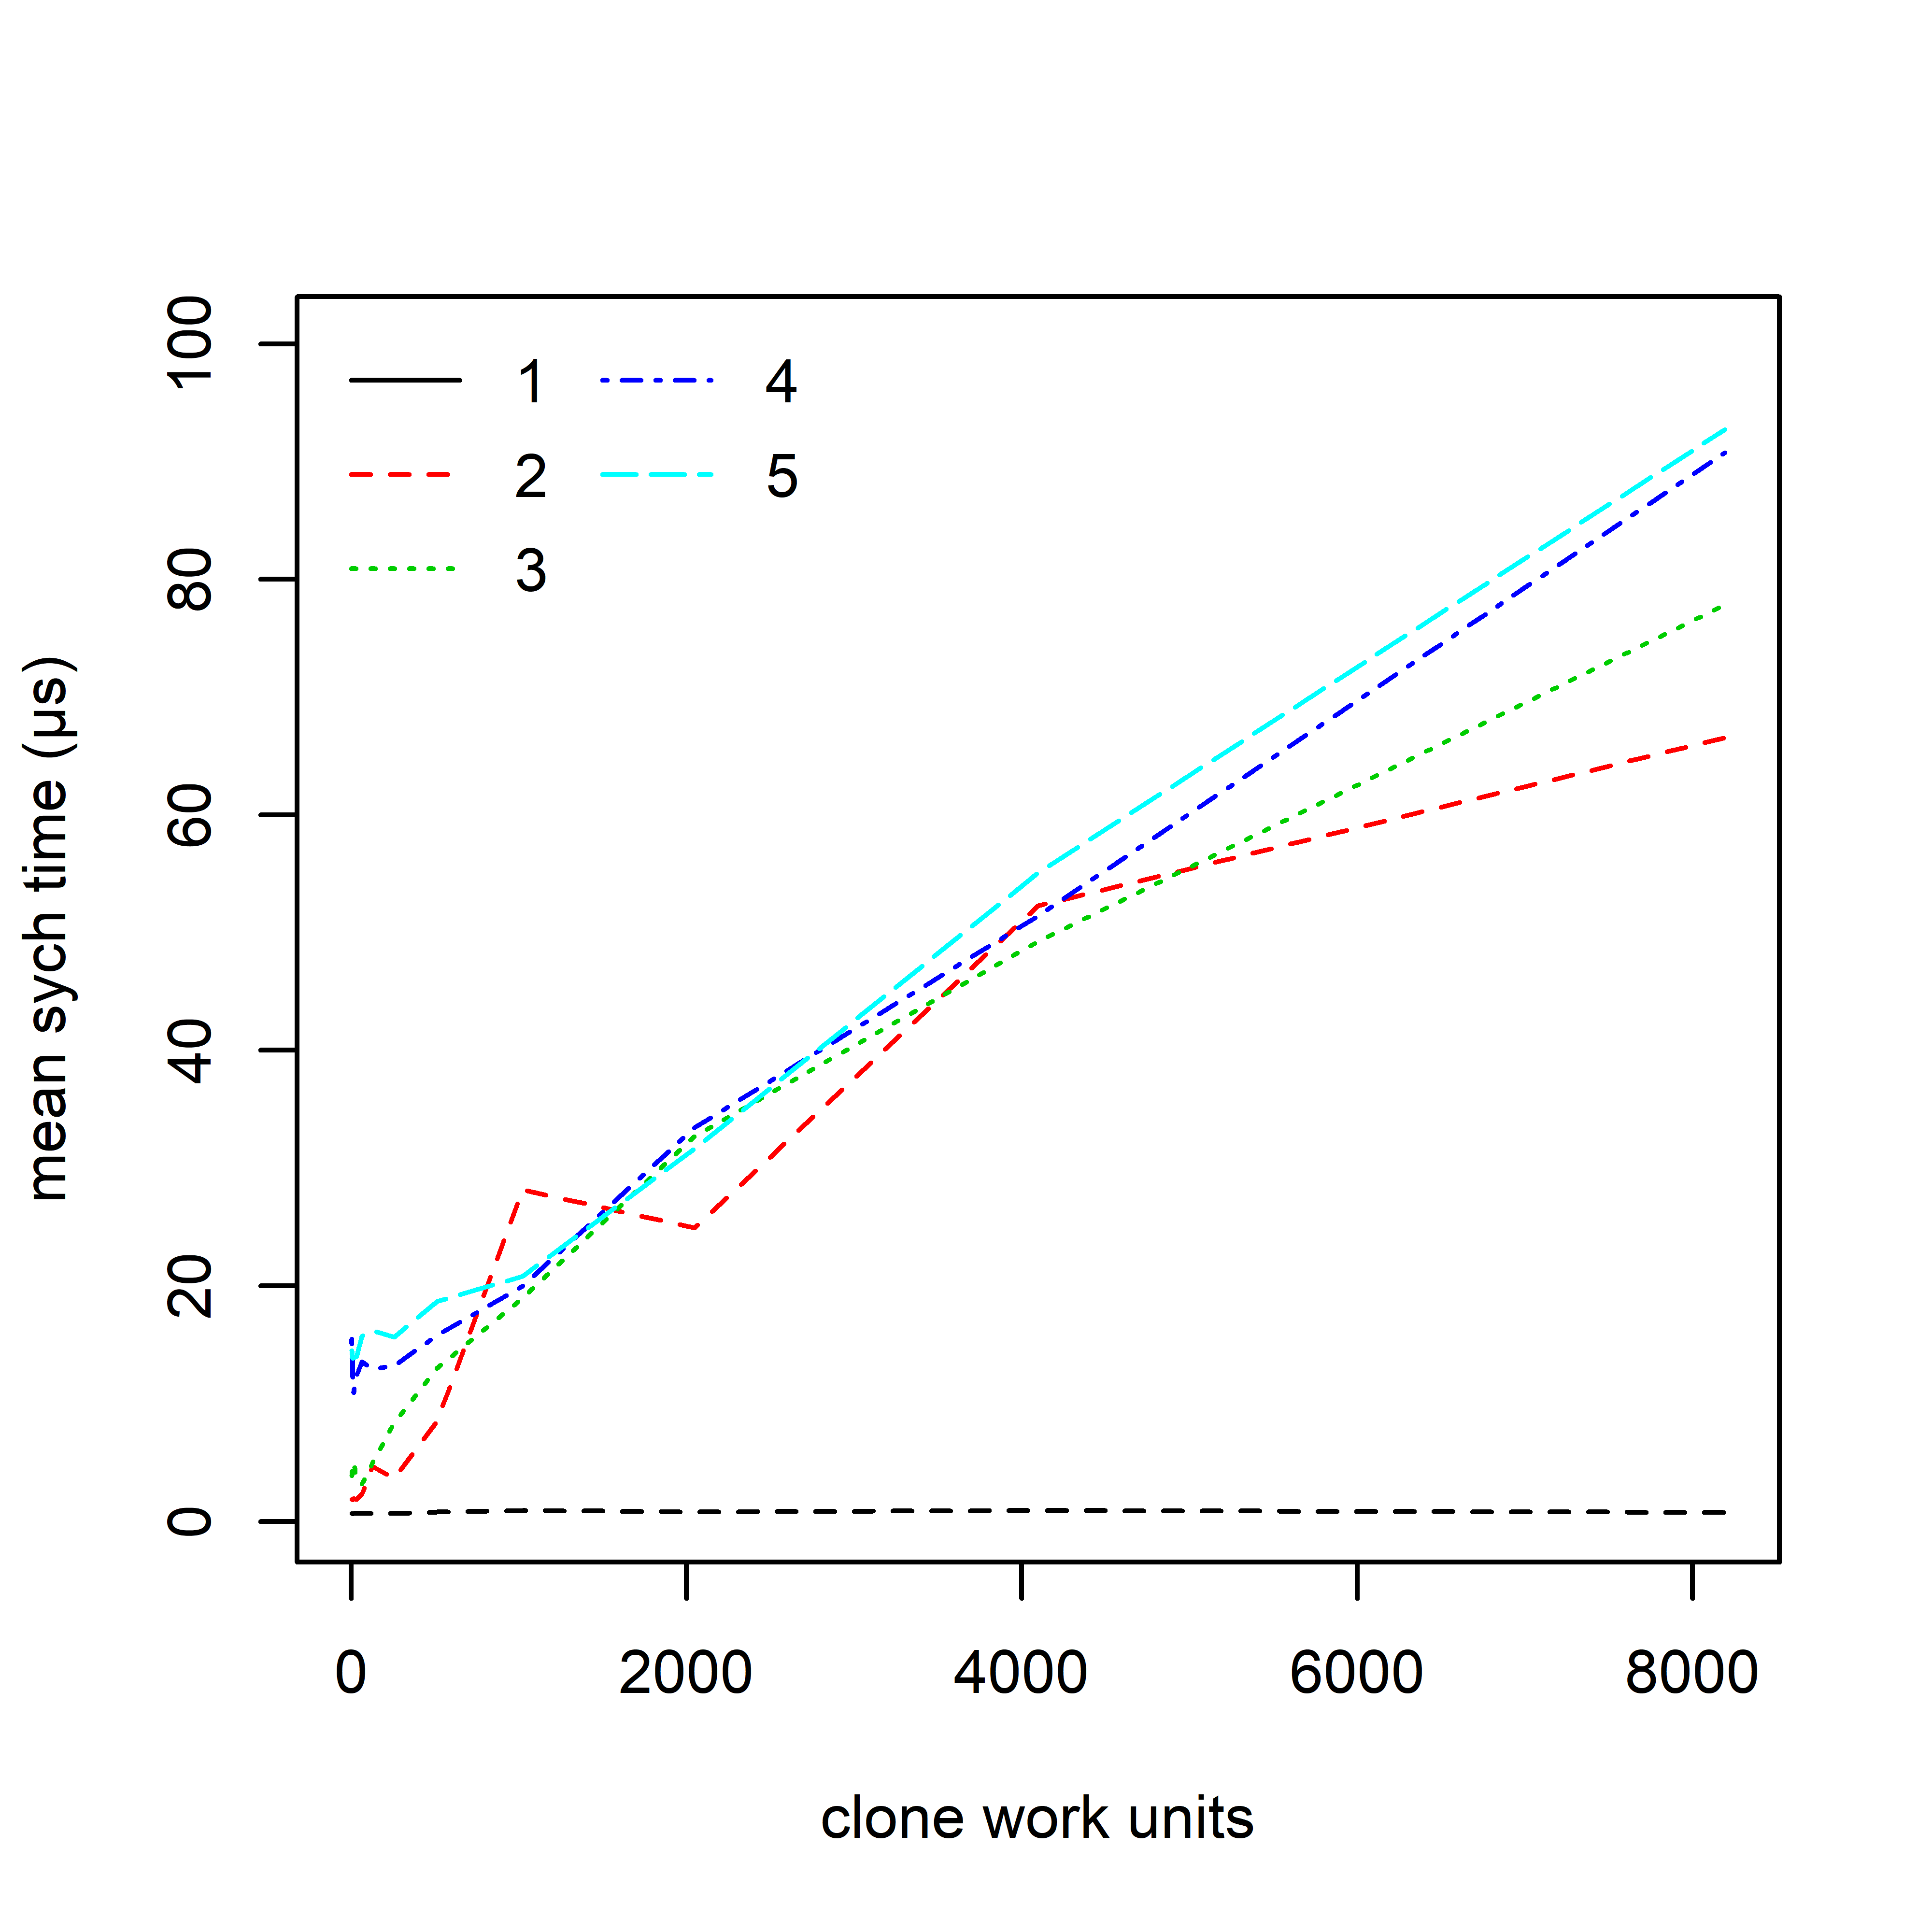
\includegraphics[width=\textwidth]{experiments/clone_compete_0.png}
		\caption{}
		\label{fig:clone_compete_0}
	\end{subfigure}%
	\begin{subfigure}[b]{0.63\textwidth}
		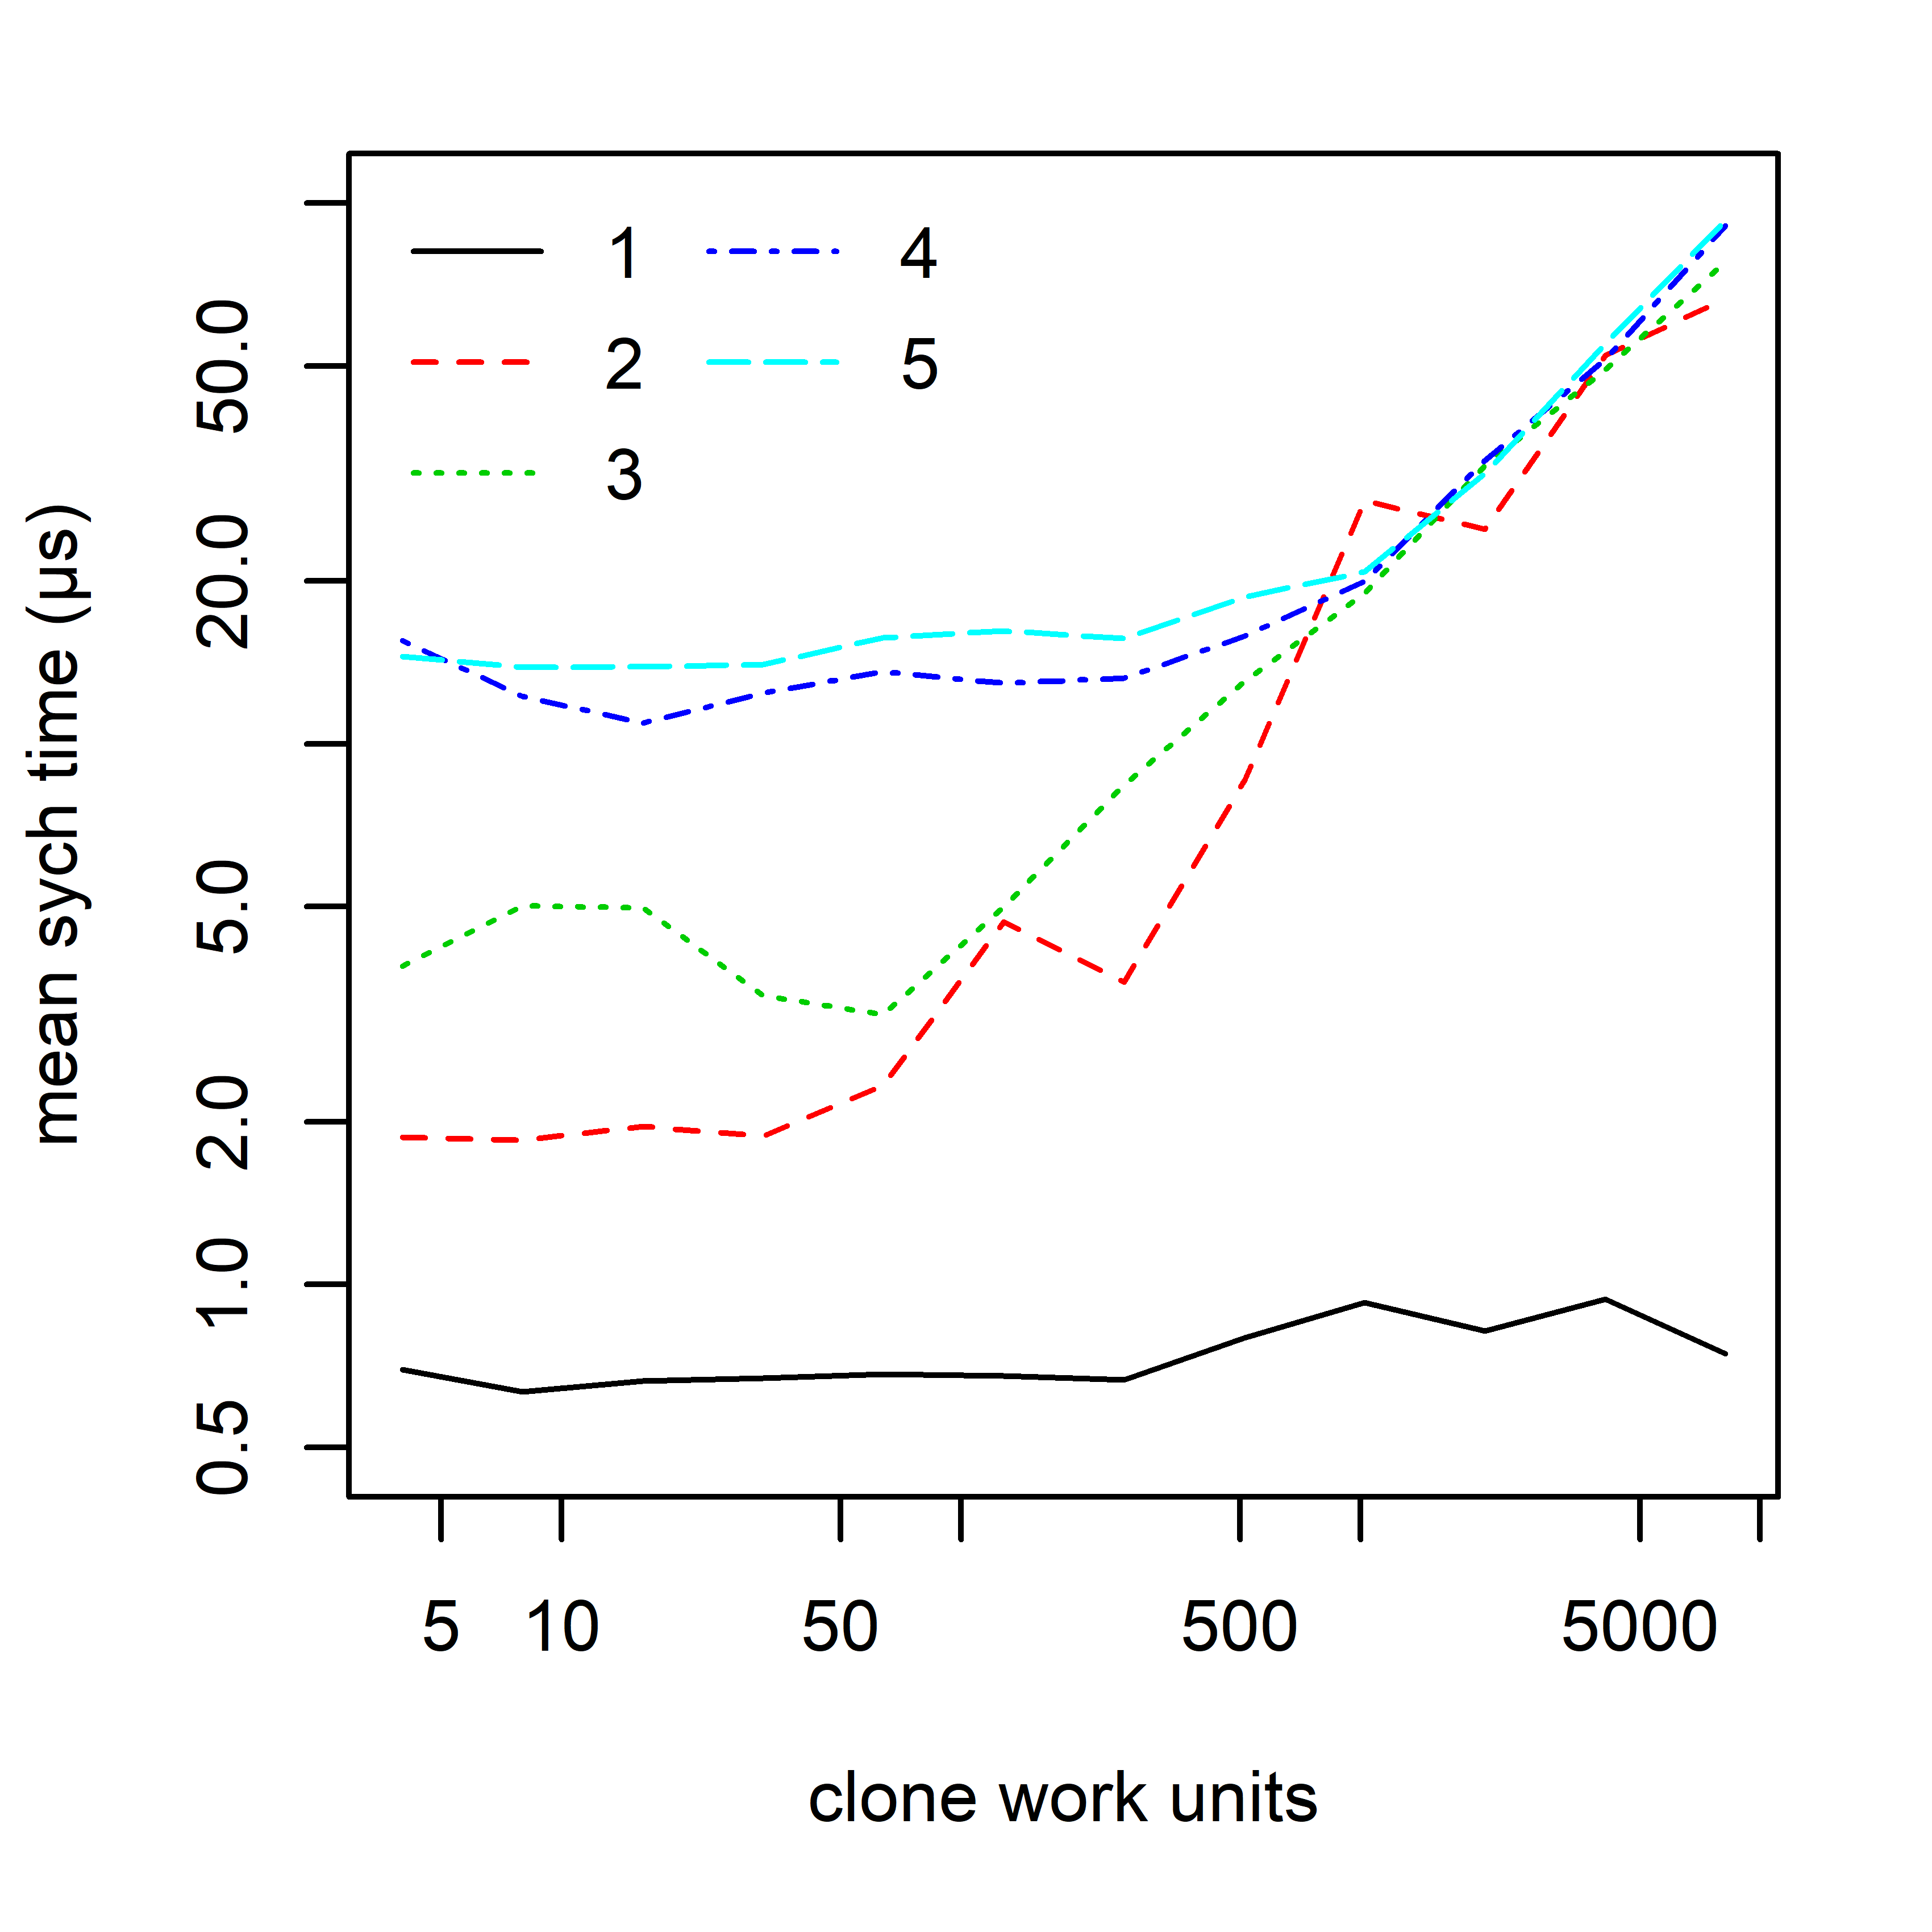
\includegraphics[width=\textwidth]{experiments/clone_compete_1.png}
		\caption{}
		\label{fig:clone_compete_1}
	\end{subfigure}%
}
\caption[TODO]{TODO.}
\label{fig:clone_compete}
\end{figure}

\begin{figure}
	\centering
	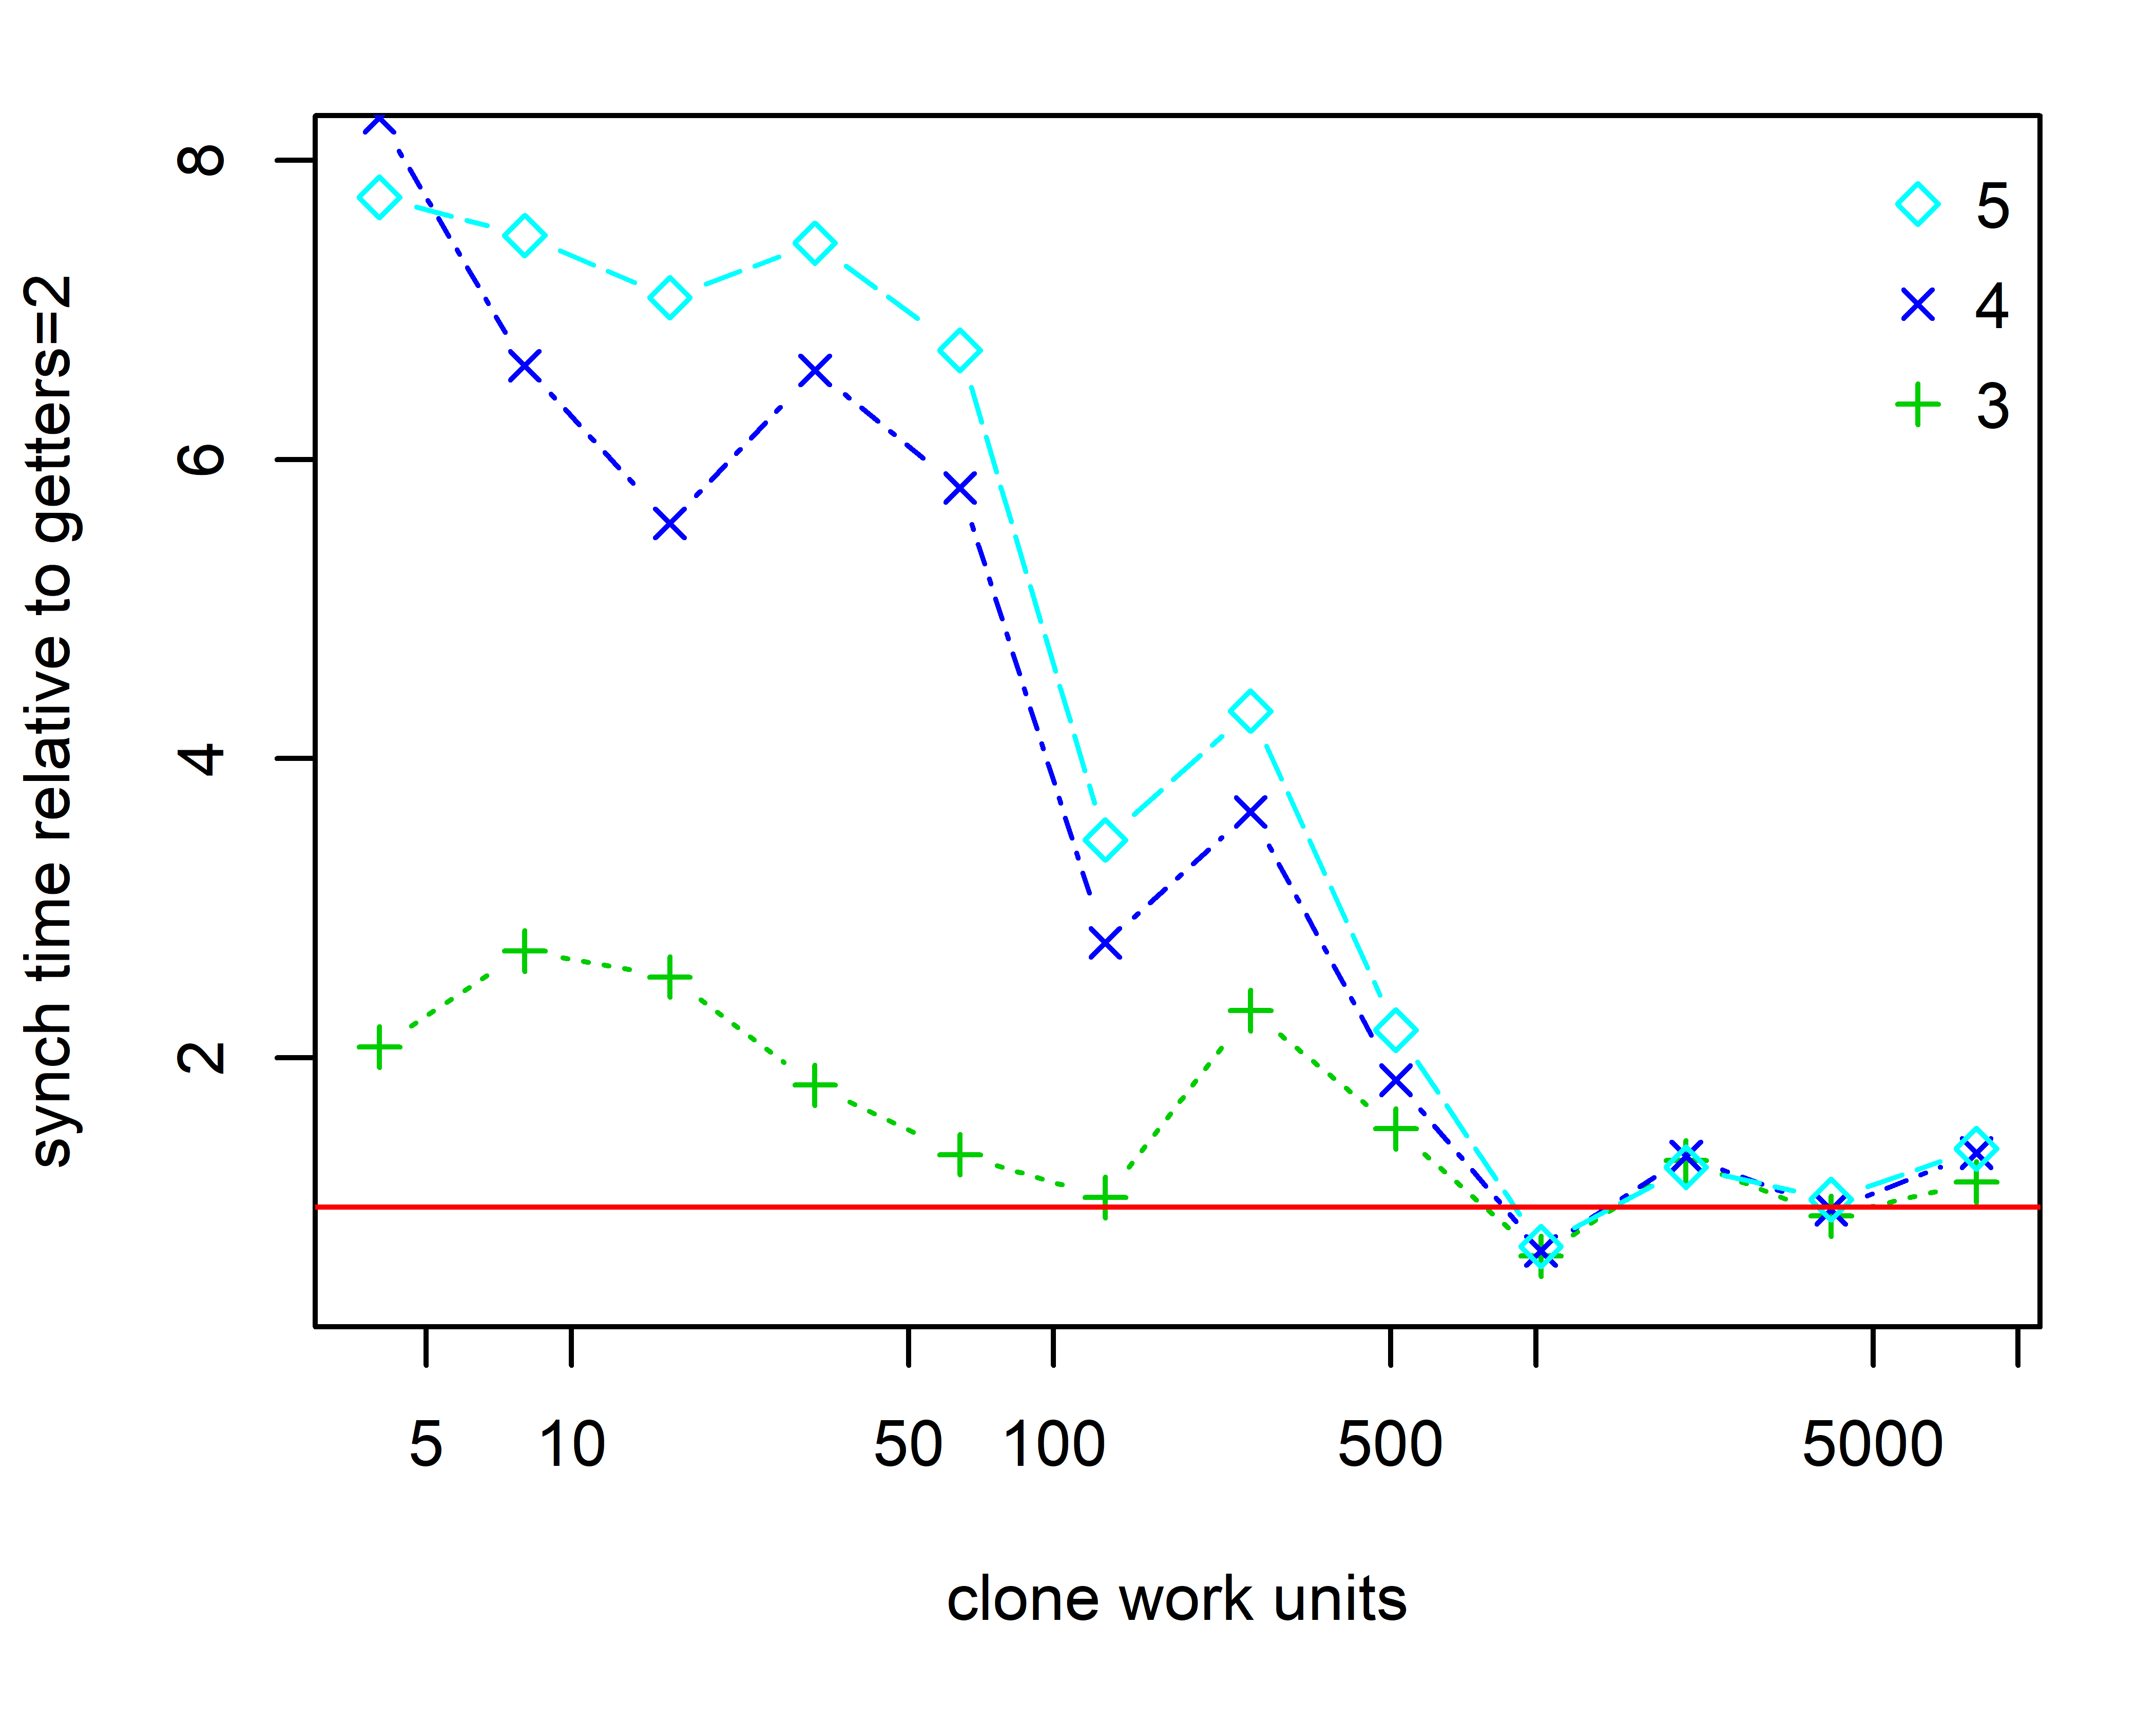
\includegraphics[width=0.8\textwidth]{experiments/clone_compete_2.png}
	\caption[TODO]{TODO.}
	\label{fig:clone_compete_3}
\end{figure}


Figure~\ref{fig:check_time} gives an overview of how long various non-firing rules add to the coordination time. here we see the round trip from the moment get is initiated to the moment it completes in a situation where always one rule can fire. we have designed it such that a number of blocked rules are always evaluated first. here we plot the time taken for each of these connectors, plotted over the number of these bogus rules encountered. we observe the expected linear scaling. The time for 0 bogus rules clearly shows the NON overhead time. non-ready guards cost 8.76 nanosec, false checks cost 18.91 ns each, 5x5 nested and checks were 180.72 each, allocations were 316.51 ns each, including freeing etc.
\begin{figure}
	\centering
	\makebox[\textwidth][c]{
		\begin{subfigure}[b]{0.63\textwidth}
			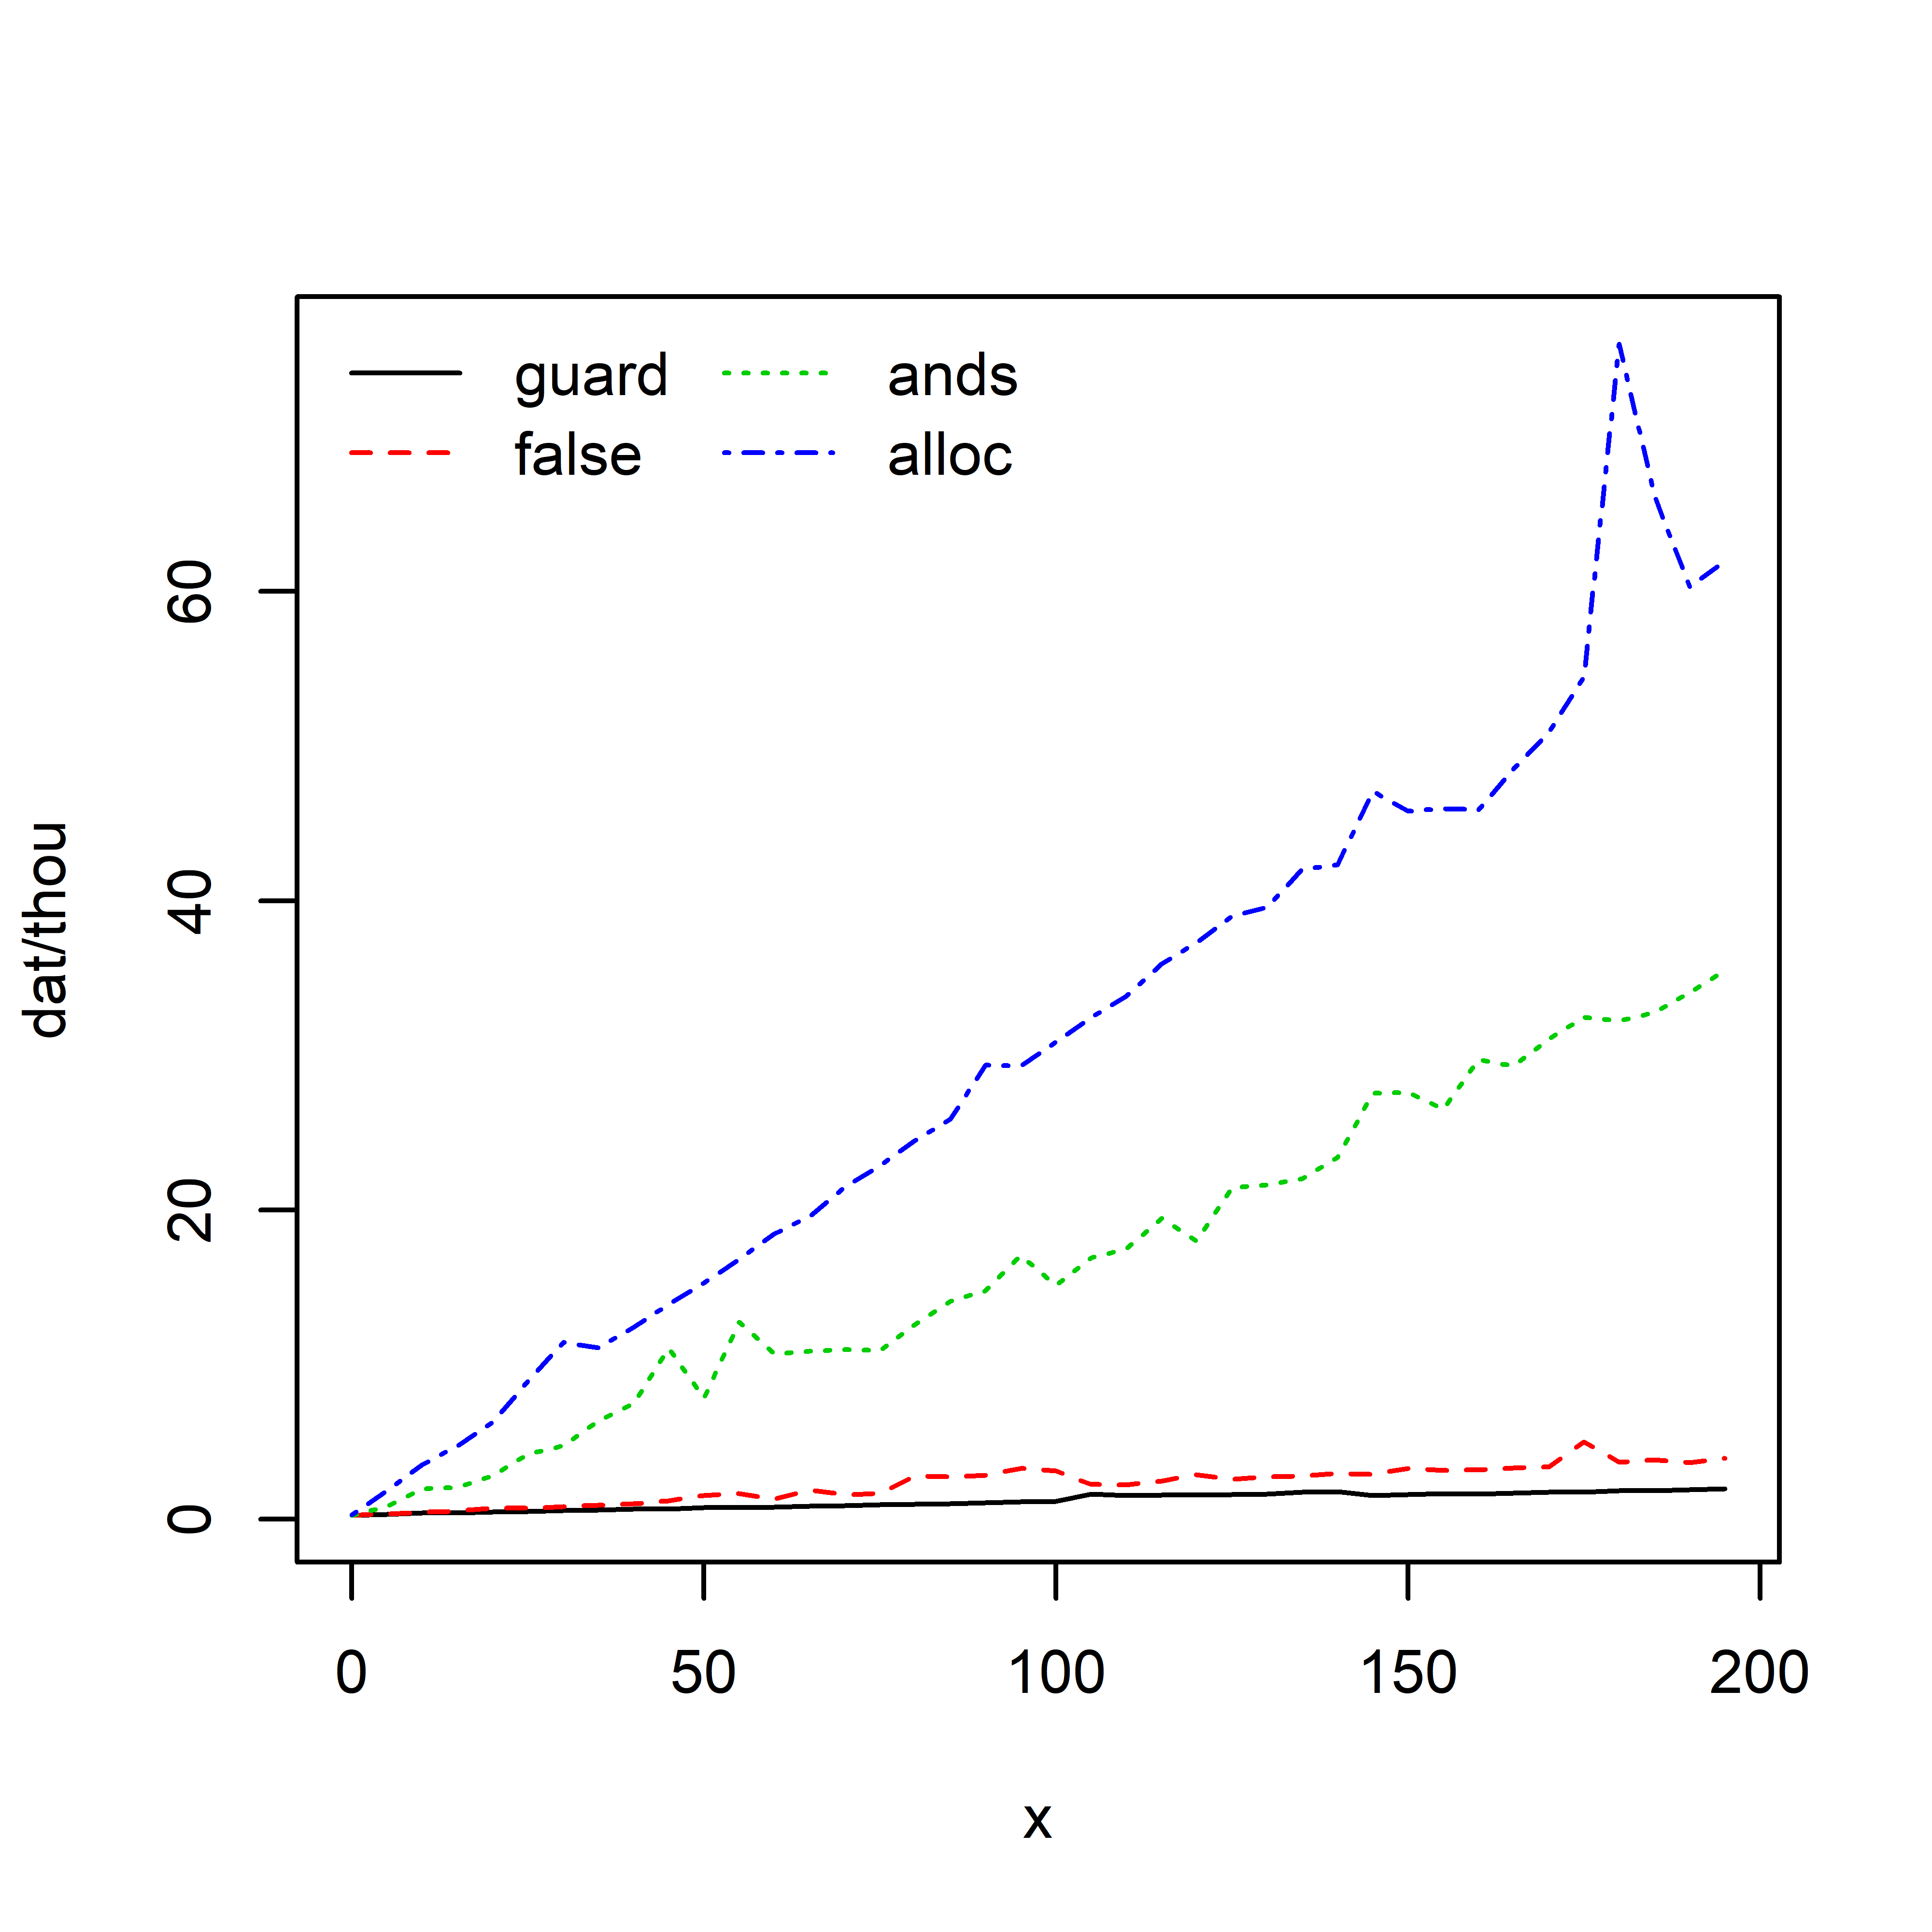
\includegraphics[width=\textwidth]{experiments/check_time_0.png}
			\caption{}
			\label{fig:check_time_0}
		\end{subfigure}%
		\begin{subfigure}[b]{0.63\textwidth}
			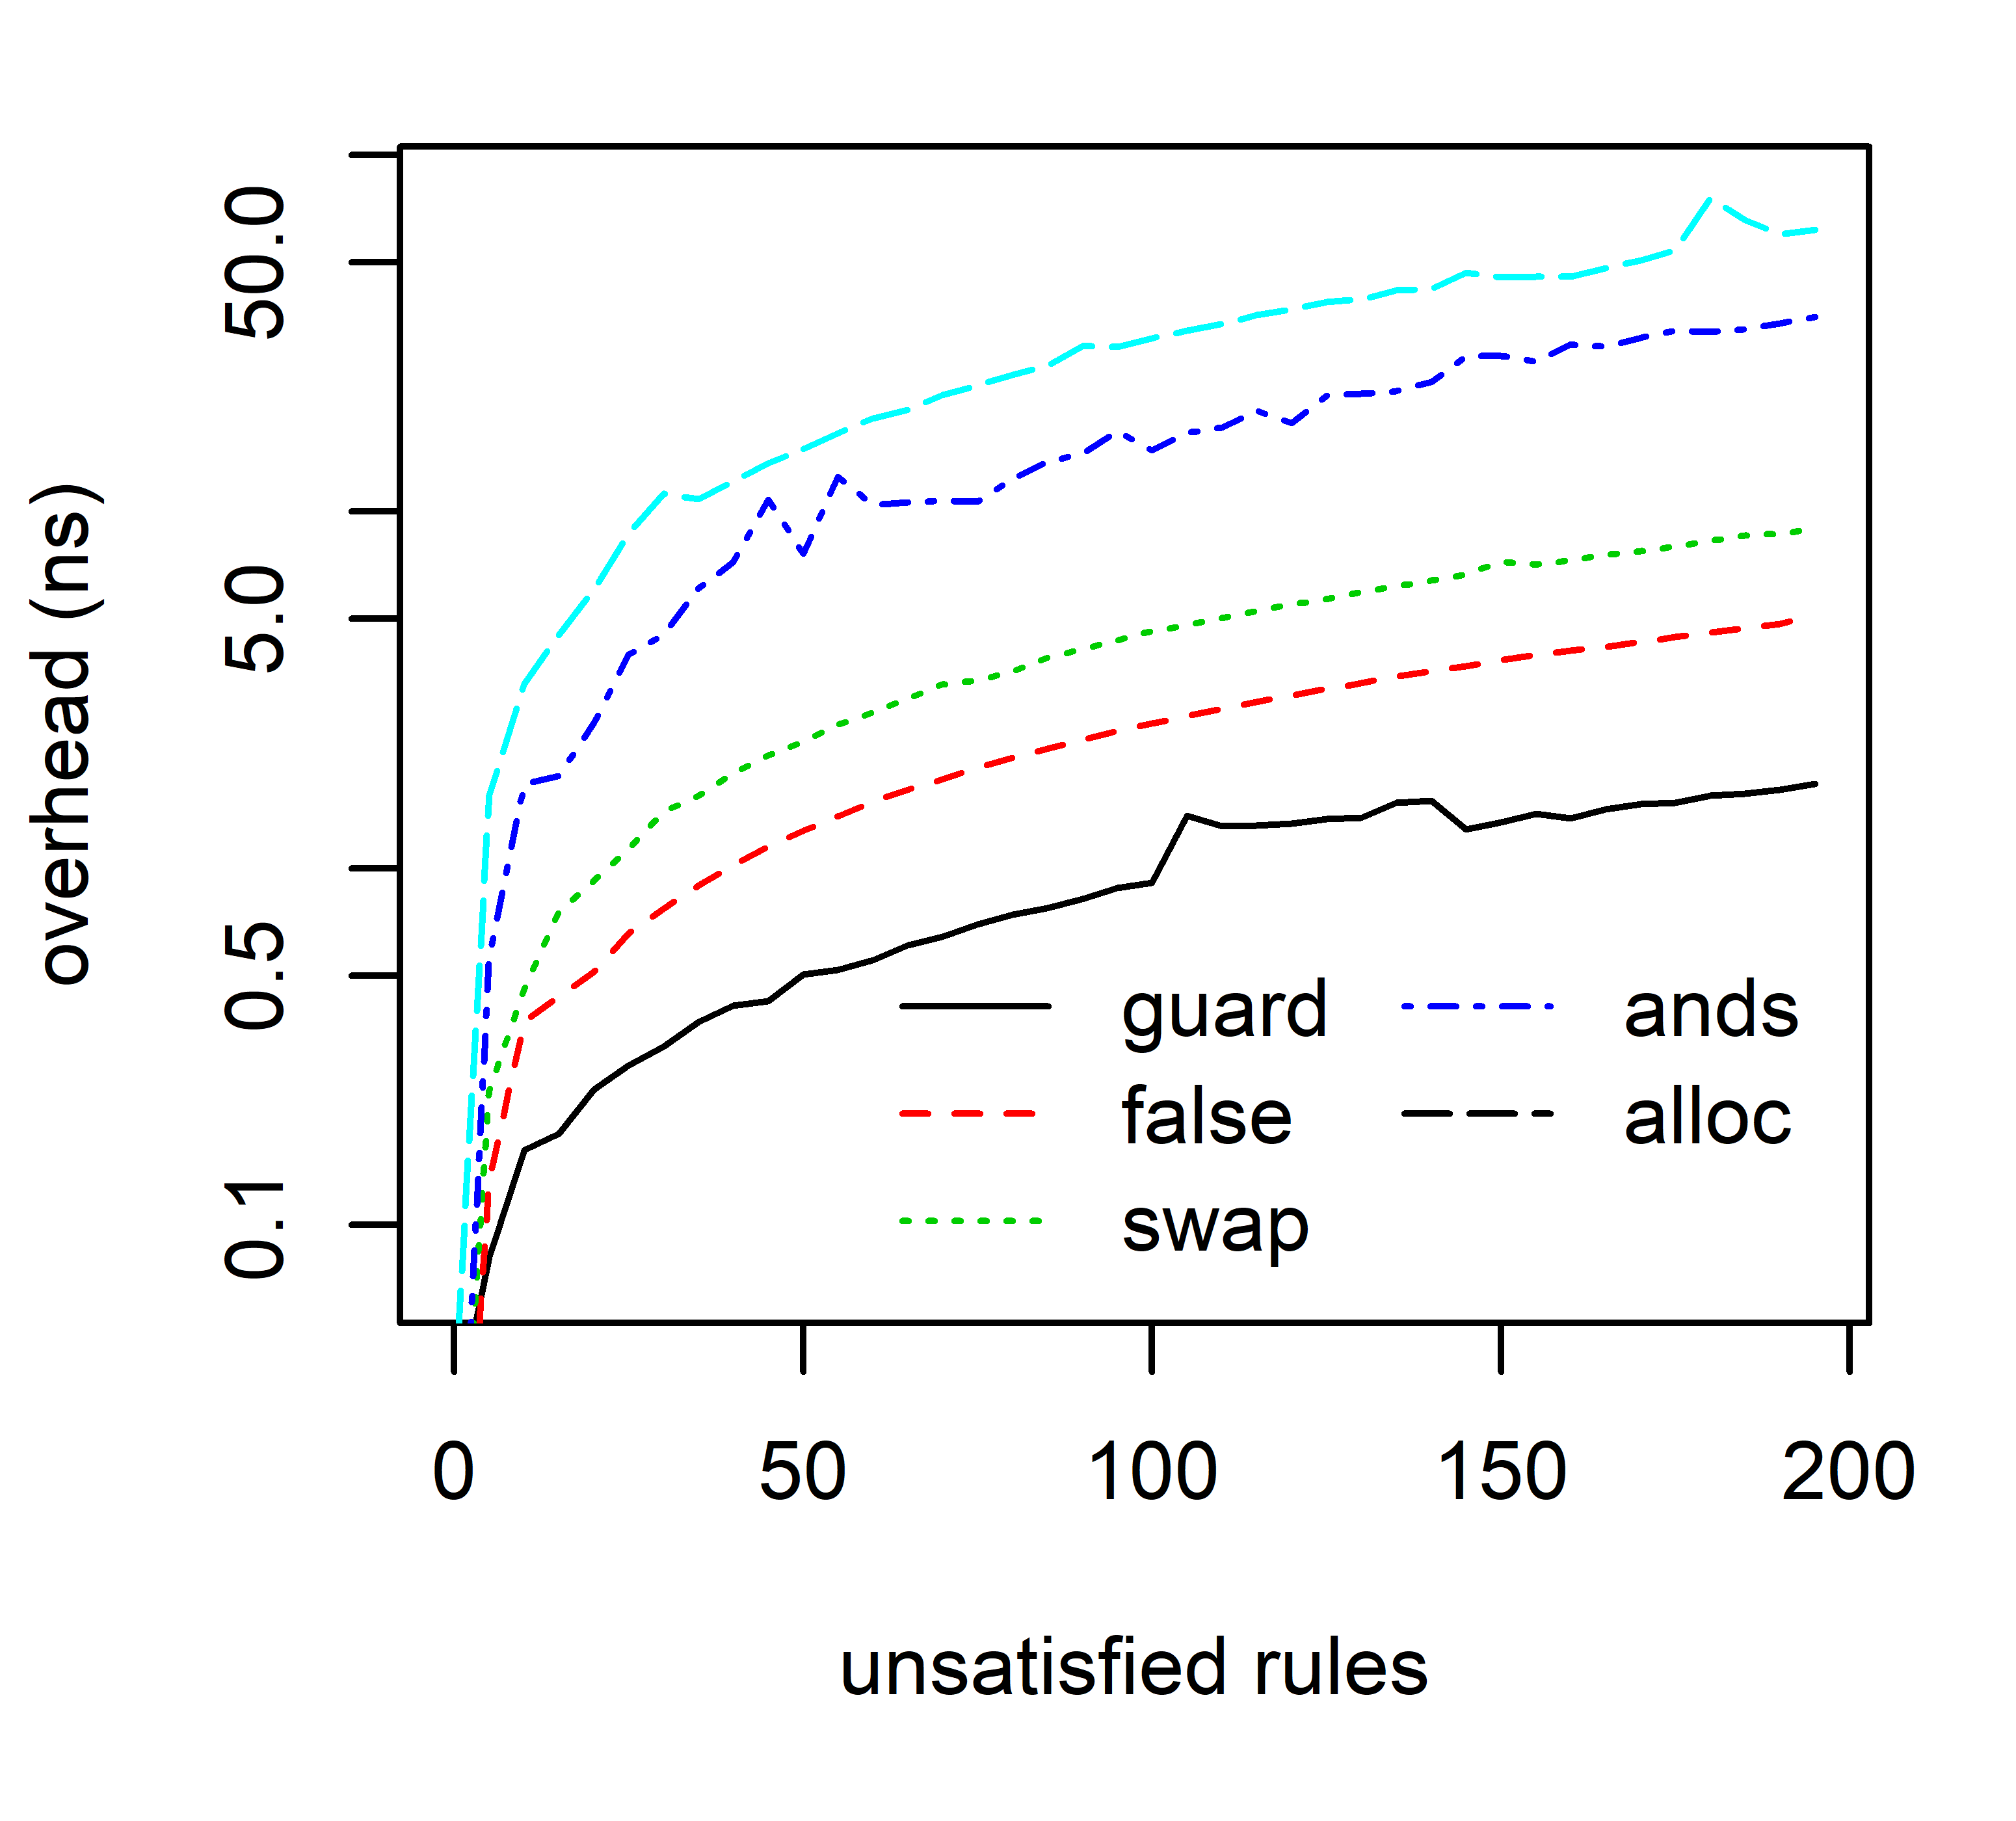
\includegraphics[width=\textwidth]{experiments/check_time_1.png}
			\caption{}
			\label{fig:check_time_2}
		\end{subfigure}%
	}
	\caption[TODO]{TODO.}
	\label{fig:check_time}
\end{figure}

%
%\begin{figure}[t]
%	\centering
%	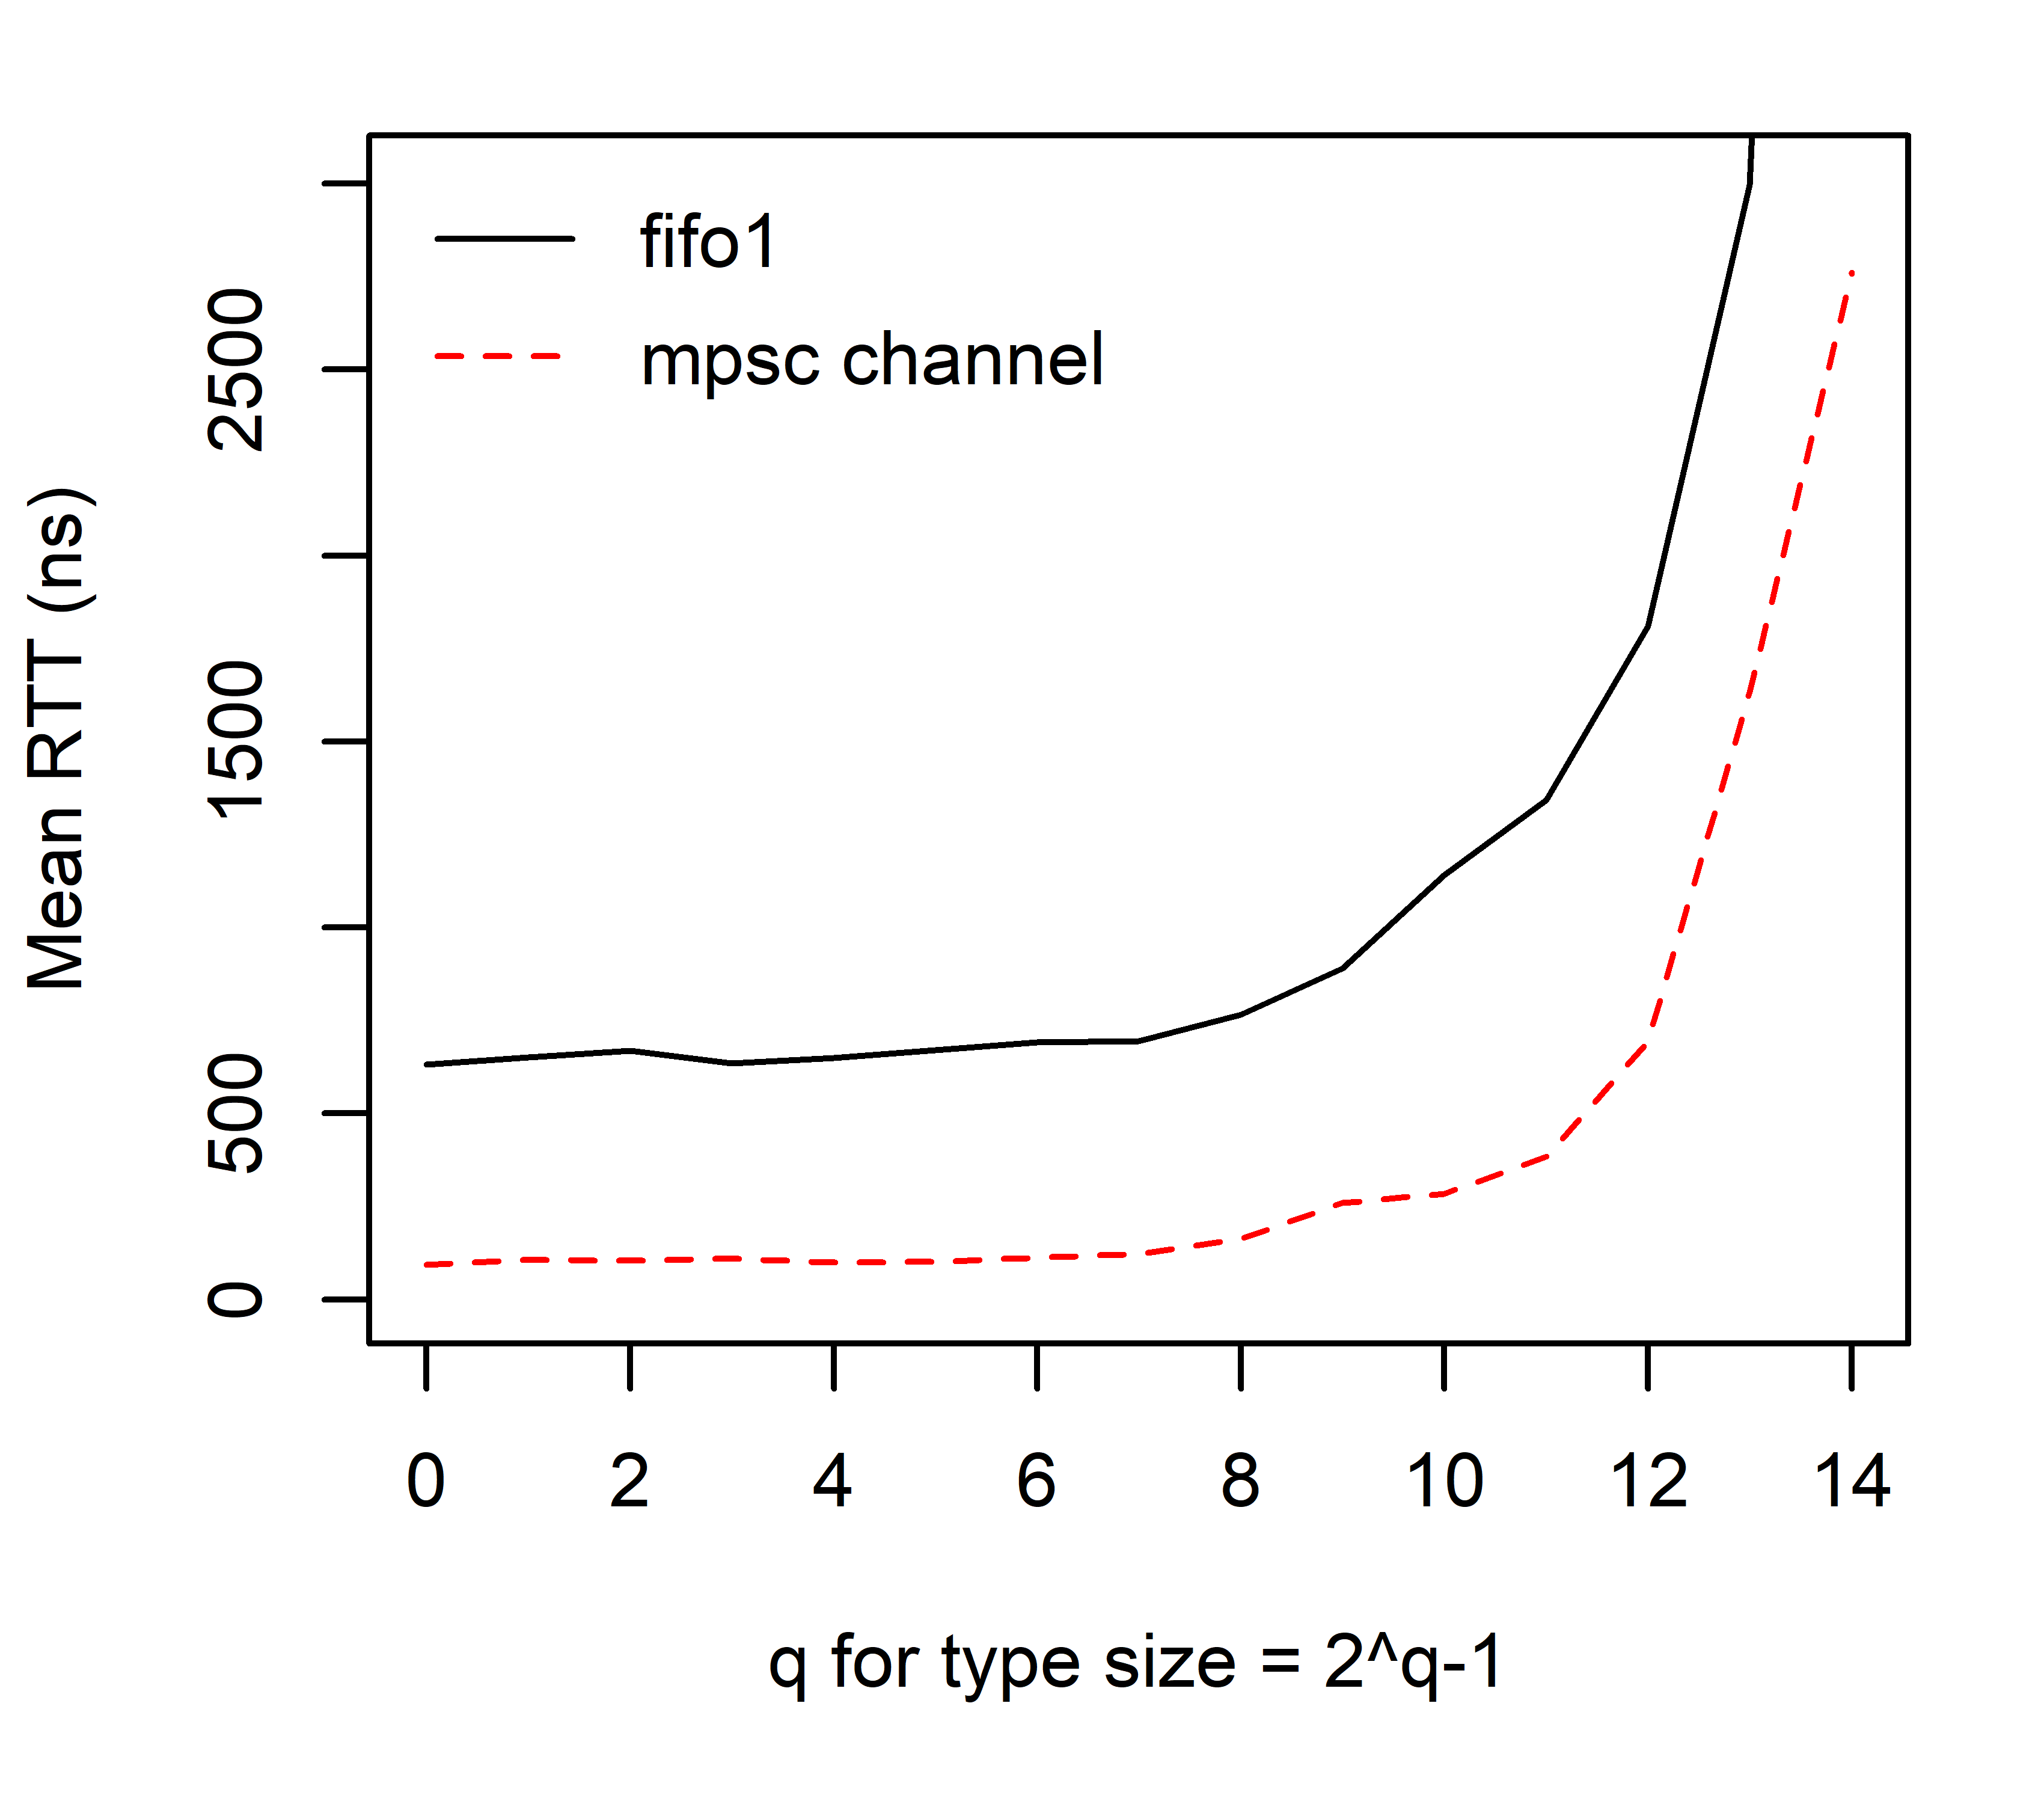
\includegraphics[width=8cm]{experiments/rtt_0.png}
%	\caption[TODO]{TODO}
%	\label{fig:exper_rtt_0}
%\end{figure}

\section{Observations}